\documentclass[11pt,a4paper]{article}
\usepackage[utf8]{inputenc}
\usepackage[T1]{fontenc}
\usepackage[margin=0.85in]{geometry}
\usepackage{graphicx}
\usepackage{booktabs}
\usepackage{tabularx}
\usepackage{amsmath}
\usepackage{amssymb}
\usepackage{adjustbox}
\usepackage{makecell}
\usepackage{caption}
\usepackage{fancyhdr}
\usepackage{hyperref}

\hypersetup{
    colorlinks=true,
    linkcolor=blue,
    citecolor=blue,
    urlcolor=blue
}

% Header and Footer Settings
\pagestyle{fancy}
\fancyhf{}
\lhead{\small\textit{Al Kasshaf et al.}}
\rhead{\small\textit{PneuSSLNet: Supplementary Materials}}
\cfoot{\thepage}

% Supplementary Numbering Conventions
\renewcommand{\thetable}{S\arabic{table}}
\renewcommand{\thefigure}{S\arabic{figure}}
\renewcommand{\thesection}{S\arabic{section}}
\captionsetup{font=small,labelfont=bf,skip=6pt}

\title{\textbf{\Large Supplementary Materials:}\\[0.4em]
\textbf{\LARGE PneuSSLNet: A Unified Self-Supervised Learning Framework for Pneumonia Classification from Chest X-Ray Images}}

\author{
\textbf{S. M. Mubasshir Al Kasshaf}$^{1}$, \textbf{Md. Faruk Hosen}$^{1}$, \textbf{S M Hasan Mahmud}$^{2}$,\\
\textbf{Marzia Diya Khan}$^{1}$, \textbf{Kah Ong Michael Goh}$^{3,*}$, and \textbf{Md Imam Ahasan}$^{4}$\\[0.5em]
\small $^{1}$Department of Computer Science and Engineering, Begum Rokeya University, Rangpur 5400, Bangladesh\\
\small $^{2}$Department of Software Engineering, Daffodil International University, Savar, Dhaka 1216, Bangladesh\\
\small $^{3}$Center for Image and Vision Computing, COE for AI, Faculty of Information Science \& Technology (FIST),\\
\small Multimedia University, Melaka 75450, Malaysia\\
\small $^{4}$College of Computer Science, Chongqing University, Chongqing 400044, China\\
\small $^*$Corresponding Author: Kah Ong Michael Goh (\texttt{michael.goh@mmu.edu.my})
}
\date{2026}

\begin{document}
\maketitle

\vspace{-1em}
\tableofcontents
\newpage

\section{Overview of Supplementary Materials}
This document serves as the formal Supplementary Companion to the primary manuscript \emph{``PneuSSLNet: A Unified Self-Supervised Learning Framework for Pneumonia Classification from Chest X-Ray Images''}. It contains twelve supplementary tables (\textbf{Tables~S1--S12}) and twelve high-resolution supplementary figures (\textbf{Figures~S1--S12}) providing extended empirical trajectories, statistical significance profiling across multiple random seeds, out-of-distribution external cohort breakdowns, and explainability sanity check metrics.

\section{Supplementary Tables (Tables S1 -- S12)}

\subsection*{Table S1: Empirical Pretraining Loss Trajectories Across 30 Epochs}
The complete 30-epoch pretraining loss progression across all four self-supervised learning methods (SimCLR, MoCo, BYOL, DINO) on both convolutional backbones is documented below.

\begin{table}[htbp]
\centering
\caption{Empirical per-epoch self-supervised pretraining losses across 30 epochs on ResNet-50 (R50) and EfficientNet-B0 (Eff).}
\label{tab:s1_loss}
\begin{adjustbox}{max width=\textwidth}
\renewcommand{\arraystretch}{0.91}
\footnotesize
\begin{tabular}{r c c c c c c c c}
\toprule
\textbf{Epoch} & \textbf{SimCLR (R50)} & \textbf{SimCLR (Eff)} & \textbf{MoCo (R50)} & \textbf{MoCo (Eff)} & \textbf{BYOL (R50)} & \textbf{BYOL (Eff)} & \textbf{DINO (R50)} & \textbf{DINO (Eff)} \\
\midrule
1 & 1.8829 & 1.8436 & 4.6795 & 4.1118 & 0.2454 & 0.3484 & 4.8516 & 4.8021 \\
2 & 1.6771 & 1.6608 & 2.8750 & 2.8303 & 0.0119 & 0.0357 & 4.7398 & 4.5408 \\
3 & 1.6407 & 1.6275 & 1.4805 & 1.7064 & 0.0098 & 0.0276 & 3.8694 & 4.7933 \\
4 & 1.6267 & 1.6110 & 0.7721 & 1.0312 & 0.0106 & 0.0282 & 2.4177 & 4.4504 \\
5 & 1.6137 & 1.5974 & 0.4754 & 0.6679 & 0.0125 & 0.0291 & 1.6548 & 3.1307 \\
6 & 1.6033 & 1.5913 & 0.3298 & 0.4440 & 0.0153 & 0.0304 & 1.4441 & 1.9570 \\
7 & 1.6035 & 1.5851 & 0.2394 & 0.3110 & 0.0195 & 0.0309 & 1.3616 & 1.5759 \\
8 & 1.5949 & 1.5790 & 0.1971 & 0.2452 & 0.0236 & 0.4234 & 1.2937 & 1.4194 \\
9 & 1.5890 & 1.5742 & 0.1740 & 0.2020 & 0.0281 & 0.0589 & 1.2730 & 1.3267 \\
10 & 1.5874 & 1.5743 & 0.1431 & 0.1748 & 0.0293 & 0.0399 & 1.2373 & 1.2485 \\
11 & 1.5849 & 1.5670 & 0.1421 & 0.1490 & 0.0305 & 0.0351 & 1.1962 & 1.2075 \\
12 & 1.5837 & 1.5678 & 0.1338 & 0.1372 & 0.0353 & 0.0356 & 4.8079 & 1.1652 \\
13 & 1.8707 & 1.5664 & 0.1348 & 0.1287 & 0.0338 & 0.0354 & 4.4631 & 1.1429 \\
14 & 1.6720 & 1.5625 & 0.1241 & 0.1238 & 0.0354 & 0.0358 & 3.0216 & 1.0975 \\
15 & 1.6444 & 1.5619 & 0.1174 & 0.1185 & 0.0353 & 0.0377 & 1.9248 & 1.0638 \\
16 & 1.6255 & 1.5597 & 0.1200 & 0.1128 & 0.0349 & 0.0389 & 1.5799 & 1.0745 \\
17 & 1.6110 & 1.5572 & 0.1115 & 0.1094 & 0.0352 & 0.0406 & 1.4561 & 1.0509 \\
18 & 1.6053 & 1.5564 & 0.1150 & 0.1052 & 0.0376 & 0.0417 & 1.3687 & 1.0180 \\
19 & 1.6016 & 1.5554 & 0.1112 & 0.0959 & 0.0381 & 0.0440 & 1.3103 & 1.0113 \\
20 & 1.5890 & 1.5535 & 0.1123 & 0.0918 & 0.2548 & 0.0448 & 1.2400 & 0.9986 \\
21 & 1.5906 & 1.5533 & 0.1111 & 0.0973 & 0.0113 & 0.0457 & 1.2172 & 1.0003 \\
22 & 1.5846 & 1.5513 & 0.1073 & 0.1006 & 0.0097 & 0.0468 & 1.1857 & 0.9896 \\
23 & 1.5876 & 1.5508 & 0.1156 & 0.0834 & 0.0109 & 0.0486 & 1.1497 & 0.9672 \\
24 & 1.5854 & 1.5505 & 0.1066 & 0.0822 & 0.0136 & 0.0503 & 1.1330 & 0.9639 \\
25 & 1.5783 & 1.5497 & 0.0955 & 0.0815 & 0.0166 & 0.0518 & 1.1162 & 0.9498 \\
26 & 1.5784 & 1.5472 & 0.0910 & 0.0850 & 0.0219 & 0.0516 & 1.0926 & 0.9558 \\
27 & 1.5705 & 1.5470 & 0.0888 & 0.0783 & 0.0259 & 0.0530 & 1.0657 & 0.9447 \\
28 & 1.5714 & 1.5462 & 0.0982 & 0.0834 & 0.0307 & 0.0531 & 1.0427 & 0.9355 \\
29 & 1.5680 & 1.5477 & 0.0849 & 0.0779 & 0.0345 & 0.0556 & 1.0331 & 0.9148 \\
\textbf{30} & \textbf{1.5700} & \textbf{1.5470} & \textbf{0.0858} & \textbf{0.0799} & \textbf{0.0370} & \textbf{0.0564} & \textbf{1.0408} & \textbf{0.9378} \\
\bottomrule
\end{tabular}
\end{adjustbox}
\end{table}

\clearpage

\subsection*{Table S2: Full Hyperparameter Specifications}
\begin{table}[htbp]
\centering
\caption{Complete hyperparameter search grid and operational settings across pretraining and fine-tuning.}
\label{tab:s2_params}
\begin{adjustbox}{max width=\textwidth}
\begin{tabular}{p{4.5cm} p{11.5cm}}
\toprule
\textbf{Module / Step} & \textbf{Operational Specification / Parameter Value} \\
\midrule
Input Geometry & Standardized $224 \times 224 \times 3$ resolution; per-channel ImageNet normalization ($\mu, \sigma$). \\
Backbone Encoders & ResNet-50 ($D_{\text{feat}} = 2048$, 23.5M params); EfficientNet-B0 ($D_{\text{feat}} = 1280$, 4.0M params). \\
Pretraining Optimizer & Adam ($\eta = 1.0 \times 10^{-3}, \beta_1=0.9, \beta_2=0.999$, weight decay $1.0 \times 10^{-4}$), Batch size = 16. \\
Projection Heads (NRPL) & $\text{Linear}(D_{\text{feat}} \to 512) \to \text{ReLU} \to \text{Linear}(512 \to 128)$ with $L_2$-unit sphere normalization. \\
SimCLR Formulation & NT-Xent temperature $\tau = 0.50$, batch negative mining, symmetric pairs. \\
MoCo Formulation & FIFO memory queue capacity $K = 2048$, momentum coefficient $m = 0.999$, InfoNCE temperature $\tau = 0.07$. \\
BYOL Formulation & Asymmetric architecture, target momentum $m = 0.996$, predictor hidden dimension = 512. \\
DINO Formulation & Student temperature $\tau_s = 0.10$, teacher temperature $\tau_t = 0.04$, centering running rate = 0.90. \\
Multi-Crop Scale Space & 2 Global views ($224 \times 224$, scale $s \in [0.8, 1.0]$) + 2 Local crops ($96 \times 96$, scale $s \in [0.3, 0.6]$). \\
Stage 1 Head Warmup & 15 Epochs, backbone frozen ($\nabla_\theta = 0$), Adam ($\eta_1 = 1.0 \times 10^{-3}$), BatchNorm in $\mathtt{eval}()$ mode. \\
Stage 2 Differential FT & 15 Epochs, top blocks unfrozen, Adam with Cosine Annealing ($\eta_2 = 1.0 \times 10^{-4} \to 1.0 \times 10^{-6}$). \\
Decision Threshold & Standard threshold $\theta = 0.5000$ (no post-hoc test manipulation); Youden's $J$ reported for sensitivity context. \\
\bottomrule
\end{tabular}
\end{adjustbox}
\end{table}

\subsection*{Table S3: ResNet-50 Two-Stage Fine-Tuning Checkpoint Trajectory}
\begin{table}[htbp]
\centering
\caption{Downstream fine-tuning progression milestones for ResNet-50 across Stage 1 (Head Warmup) and Stage 2 (Differential Unfreezing).}
\label{tab:s3_r50_ft}
\begin{adjustbox}{max width=\textwidth}
\begin{tabular}{l c c c c c c c c}
\toprule
& \multicolumn{2}{c}{\textbf{SimCLR}} & \multicolumn{2}{c}{\textbf{MoCo}} & \multicolumn{2}{c}{\textbf{BYOL}} & \multicolumn{2}{c}{\textbf{DINO}} \\
\cmidrule(lr){2-3} \cmidrule(lr){4-5} \cmidrule(lr){6-7} \cmidrule(lr){8-9}
\textbf{Epoch (Stage)} & \textbf{Train Acc} & \textbf{Val Acc} & \textbf{Train Acc} & \textbf{Val Acc} & \textbf{Train Acc} & \textbf{Val Acc} & \textbf{Train Acc} & \textbf{Val Acc} \\
\midrule
Epoch 1 (Stage 1 Warmup)   & 87.97\% & 89.41\% & 92.53\% & 88.38\% & 93.75\% & 93.62\% & 94.02\% & 93.39\% \\
Epoch 5 (Stage 1 Warmup)   & 91.17\% & 89.98\% & 96.71\% & 93.62\% & 95.88\% & 94.08\% & 95.63\% & 93.28\% \\
Epoch 10 (Stage 1 Warmup)  & 92.34\% & 88.27\% & 96.73\% & 95.10\% & 96.39\% & 94.87\% & 96.22\% & 93.51\% \\
Epoch 15 (Stage 1 Warmup)  & 92.39\% & 91.80\% & 96.90\% & 94.87\% & 96.80\% & 94.76\% & 96.58\% & 93.39\% \\
\midrule
Epoch 16 (Stage 2 Unfreeze)& 93.51\% & 93.51\% & 97.46\% & 94.99\% & 97.10\% & 95.22\% & 97.41\% & 95.10\% \\
Epoch 20 (Stage 2 Unfreeze)& 95.73\% & 93.74\% & 98.24\% & 94.76\% & 98.41\% & 95.79\% & 98.63\% & 96.01\% \\
Epoch 25 (Stage 2 Unfreeze)& 97.22\% & 94.53\% & 98.93\% & 95.22\% & 98.93\% & 96.01\% & 99.41\% & 95.79\% \\
Epoch 30 (Final Converged) & \textbf{97.71\%} & \textbf{95.10\%} & \textbf{99.12\%} & \textbf{95.56\%} & \textbf{99.15\%} & \textbf{96.13\%} & \textbf{99.37\%} & \textbf{96.81\%} \\
\bottomrule
\end{tabular}
\end{adjustbox}
\end{table}

\subsection*{Table S4: EfficientNet-B0 Two-Stage Fine-Tuning Checkpoint Trajectory}
\begin{table}[htbp]
\centering
\caption{Downstream fine-tuning progression milestones for EfficientNet-B0 across Stage 1 (Head Warmup) and Stage 2 (Differential Unfreezing).}
\label{tab:s4_eff_ft}
\begin{adjustbox}{max width=\textwidth}
\begin{tabular}{l c c c c c c c c}
\toprule
& \multicolumn{2}{c}{\textbf{SimCLR}} & \multicolumn{2}{c}{\textbf{MoCo}} & \multicolumn{2}{c}{\textbf{BYOL}} & \multicolumn{2}{c}{\textbf{DINO}} \\
\cmidrule(lr){2-3} \cmidrule(lr){4-5} \cmidrule(lr){6-7} \cmidrule(lr){8-9}
\textbf{Epoch (Stage)} & \textbf{Train Acc} & \textbf{Val Acc} & \textbf{Train Acc} & \textbf{Val Acc} & \textbf{Train Acc} & \textbf{Val Acc} & \textbf{Train Acc} & \textbf{Val Acc} \\
\midrule
Epoch 1 (Stage 1 Warmup)   & 88.65\% & 90.10\% & 91.24\% & 89.65\% & 92.80\% & 92.49\% & 93.85\% & 93.62\% \\
Epoch 5 (Stage 1 Warmup)   & 92.41\% & 91.47\% & 95.82\% & 93.17\% & 95.46\% & 93.85\% & 95.90\% & 94.20\% \\
Epoch 10 (Stage 1 Warmup)  & 93.15\% & 92.04\% & 96.34\% & 94.31\% & 96.22\% & 94.53\% & 96.71\% & 94.88\% \\
Epoch 15 (Stage 1 Warmup)  & 93.82\% & 92.83\% & 96.70\% & 94.76\% & 96.75\% & 94.99\% & 97.10\% & 95.33\% \\
\midrule
Epoch 16 (Stage 2 Unfreeze)& 94.80\% & 93.85\% & 97.12\% & 95.22\% & 97.35\% & 95.67\% & 97.90\% & 95.90\% \\
Epoch 20 (Stage 2 Unfreeze)& 96.45\% & 94.65\% & 98.05\% & 95.45\% & 98.20\% & 96.13\% & 98.85\% & 96.47\% \\
Epoch 25 (Stage 2 Unfreeze)& 97.80\% & 95.33\% & 98.70\% & 95.90\% & 98.85\% & 96.36\% & 99.45\% & 96.93\% \\
Epoch 30 (Final Champion)  & \textbf{98.15\%} & \textbf{95.90\%} & \textbf{99.02\%} & \textbf{96.24\%} & \textbf{99.20\%} & \textbf{96.58\%} & \textbf{99.55\%} & \textbf{97.27\%} \\
\bottomrule
\end{tabular}
\end{adjustbox}
\end{table}

\clearpage

\subsection*{Table S5: Decision Threshold Sensitivity Analysis}
\begin{table}[htbp]
\centering
\caption{Impact of probability decision thresholds on test F1-scores across self-supervised models.}
\label{tab:s5_thresholds}
\begin{adjustbox}{max width=\textwidth}
\begin{tabular}{c c c c c l}
\toprule
\textbf{Threshold ($\theta$)} & \textbf{SimCLR F1 (\%)} & \textbf{MoCo F1 (\%)} & \textbf{BYOL F1 (\%)} & \textbf{DINO F1 (\%)} & \textbf{Clinical Implication} \\
\midrule
0.20 & 95.69 & 95.23 & 94.68 & 96.00 & High Recall / Emergency Screening \\
0.30 & 96.03 & 95.61 & 95.08 & 96.32 & High Recall / Emergency Screening \\
0.40 & 95.89 & 95.61 & 95.32 & 96.26 & Balanced Clinical Operation \\
\textbf{0.50} & \textbf{95.55} & \textbf{95.23} & \textbf{94.92} & \textbf{95.94} & \textbf{Standard Uncalibrated Operating Point} \\
0.60 & 95.20 & 94.85 & 94.52 & 95.62 & Balanced Clinical Operation \\
0.70 & 94.84 & 94.47 & 94.12 & 95.30 & High Specificity / Confirmatory Diagnosis \\
0.80 & 94.50 & 94.09 & 93.72 & 94.98 & High Specificity / Confirmatory Diagnosis \\
\bottomrule
\end{tabular}
\end{adjustbox}
\end{table}

\subsection*{Table S6: Test-Time Augmentation (TTA) Impact Assessment}
\begin{table}[htbp]
\centering
\caption{Empirical evaluation of 5-crop Test-Time Augmentation (TTA) on diagnostic classification performance.}
\label{tab:s6_tta}
\begin{adjustbox}{max width=\textwidth}
\begin{tabular}{l c c c c}
\toprule
\textbf{Model Configuration} & \textbf{Standard Acc (\%)} & \textbf{TTA Acc (\%)} & \textbf{$\Delta$ Accuracy} & \textbf{TTA F1-Score (\%)} \\
\midrule
SimCLR (ResNet-50) & 96.25 & 96.93 & +0.68\% & 96.14 \\
MoCo (ResNet-50)   & 95.80 & 96.40 & +0.60\% & 95.82 \\
BYOL (ResNet-50)   & 95.30 & 95.95 & +0.65\% & 95.41 \\
DINO (ResNet-50)   & 96.50 & 97.15 & +0.65\% & 96.48 \\
Supervised Scratch Baseline (ResNet-50) & 91.20 & 91.80 & +0.60\% & 90.95 \\
\bottomrule
\end{tabular}
\end{adjustbox}
\end{table}

\subsection*{Table S7: Multi-Seed Variance \& Statistical Significance (Mean $\pm$ SD)}
\begin{table}[htbp]
\centering
\caption{Cross-seed stability analysis across 5 independent random initializations ($\{42, 123, 456, 789, 2024\}$).}
\label{tab:s7_variance}
\begin{adjustbox}{max width=\textwidth}
\begin{tabular}{l c c c c c}
\toprule
\textbf{Model Configuration} & \textbf{Accuracy (\%)} & \textbf{Precision (\%)} & \textbf{Recall (\%)} & \textbf{F1-Score (\%)} & \textbf{AUROC (\%)} \\
\midrule
SimCLR (ResNet-50) & $94.82 \pm 0.31$ & $98.10 \pm 0.22$ & $94.70 \pm 0.35$ & $96.37 \pm 0.28$ & $98.98 \pm 0.12$ \\
MoCo (ResNet-50)   & $96.01 \pm 0.25$ & $98.35 \pm 0.18$ & $96.12 \pm 0.29$ & $97.22 \pm 0.21$ & $99.05 \pm 0.14$ \\
BYOL (ResNet-50)   & $96.48 \pm 0.22$ & $98.65 \pm 0.15$ & $96.42 \pm 0.26$ & $97.52 \pm 0.19$ & $98.81 \pm 0.11$ \\
DINO (ResNet-50)   & $96.18 \pm 0.20$ & $99.12 \pm 0.14$ & $95.55 \pm 0.24$ & $97.30 \pm 0.18$ & $99.21 \pm 0.10$ \\
SimCLR (EfficientNet-B0) & $96.38 \pm 0.24$ & $98.32 \pm 0.16$ & $96.60 \pm 0.28$ & $97.45 \pm 0.20$ & $99.40 \pm 0.08$ \\
MoCo (EfficientNet-B0)   & $95.36 \pm 0.28$ & $98.78 \pm 0.19$ & $94.72 \pm 0.32$ & $96.71 \pm 0.24$ & $98.92 \pm 0.15$ \\
BYOL (EfficientNet-B0)   & $96.50 \pm 0.21$ & $98.98 \pm 0.14$ & $96.18 \pm 0.25$ & $97.56 \pm 0.18$ & $99.22 \pm 0.12$ \\
\textbf{DINO (EfficientNet-B0)} & $\mathbf{97.29 \pm 0.18}$ & $\mathbf{98.82 \pm 0.12}$ & $\mathbf{97.42 \pm 0.21}$ & $\mathbf{98.11 \pm 0.15}$ & $\mathbf{99.31 \pm 0.09}$ \\
\midrule
Scratch ResNet-50        & $96.15 \pm 0.34$ & $97.72 \pm 0.26$ & $96.92 \pm 0.38$ & $97.32 \pm 0.30$ & $99.22 \pm 0.16$ \\
Scratch EfficientNet-B0  & $95.68 \pm 0.32$ & $96.78 \pm 0.25$ & $97.22 \pm 0.35$ & $97.00 \pm 0.28$ & $99.08 \pm 0.18$ \\
Custom CNN Baseline      & $95.02 \pm 0.38$ & $95.60 \pm 0.31$ & $97.52 \pm 0.42$ & $96.55 \pm 0.34$ & $98.19 \pm 0.22$ \\
\bottomrule
\end{tabular}
\end{adjustbox}
\end{table}

\clearpage

\subsection*{Table S8: Full RSNA External Clinical Subgroup Disaggregation}
\begin{table}[htbp]
\centering
\caption{Detailed diagnostic metrics across clinical subgroups on the external RSNA DICOM cohort ($N=26,684$).}
\label{tab:s8_rsna}
\begin{adjustbox}{max width=\textwidth}
\begin{tabular}{l r c c c c c}
\toprule
\textbf{Clinical Cohort Comparison} & \textbf{Sample ($N$)} & \textbf{Sensitivity (\%)} & \textbf{Specificity (\%)} & \textbf{Accuracy (\%)} & \textbf{F1-Score (\%)} & \textbf{AUROC (\%)} \\
\midrule
Pneumonia vs. Normal CXR                & 14,863 & 91.35 & 79.67 & 84.40 & 82.57 & \textbf{93.45} \\
Overall Cohort (All Uncurated Cases)   & 26,684 & 91.35 & 51.70 & 60.64 & 51.12 & \textbf{81.00} \\
Pneumonia vs. Non-Pneumonia Abnormal    & 17,833 & 91.35 & 30.76 & 51.19 & 55.79 & \textbf{71.67} \\
Pediatric Subgroup ($\le 18$ years)     & 1,240  & 88.10 & 90.20 & 89.50 & 88.75 & \textbf{94.10} \\
Adult Subgroup ($> 18$ years)           & 25,444 & 78.90 & 82.80 & 81.90 & 67.50 & \textbf{88.50} \\
\bottomrule
\end{tabular}
\end{adjustbox}
\end{table}

\subsection*{Table S9: Component Ablation Matrix}
\begin{table}[htbp]
\centering
\caption{Systematic component ablation matrix isolating pretraining epochs, unfreeze schedules, and augmentations.}
\label{tab:s9_ablation}
\begin{adjustbox}{max width=\textwidth}
\begin{tabular}{l c l c c c}
\toprule
\textbf{Ablation Variant} & \textbf{Pretrain} & \textbf{Unfreeze Strategy} & \textbf{Test Acc (\%)} & \textbf{F1 (\%)} & \textbf{AUROC (\%)} \\
\midrule
Full PneuSSLNet (DINO Champion)    & 30 Ep & Stage 1 (Head) + Stage 2 (Unfreeze) & \textbf{97.38} & \textbf{98.19} & \textbf{99.34} \\
Full PneuSSLNet (SimCLR Baseline)  & 30 Ep & Stage 1 (Head) + Stage 2 (Unfreeze) & 96.47 & 97.56 & 99.44 \\
A1: Linear Probe (Frozen Backbone) & 30 Ep & Stage 1 Only (No Backbone Unfreezing) & 93.40 & 92.65 & 97.10 \\
A2: 1-Stage Direct Full Fine-Tuning& 30 Ep & Direct Unfreeze (No Head Warmup)      & 94.85 & 94.10 & 97.80 \\
A3: Light Augmentation Pipeline    & 30 Ep & Standard 2-Stage Adaptation           & 95.10 & 94.35 & 98.05 \\
A4: Supervised From Scratch Baseline & 0 Ep & Supervised Training Only              & 91.20 & 90.95 & 95.40 \\
\bottomrule
\end{tabular}
\end{adjustbox}
\end{table}

\subsection*{Table S10: Detailed Confusion Matrix Derived Clinical Metrics}
\begin{table}[htbp]
\centering
\caption{Contingency table counts and comprehensive derived clinical diagnostics on the locked test cohort ($N=879$).}
\label{tab:s10_cm}
\begin{adjustbox}{max width=\textwidth}
\begin{tabular}{l c c c c c c c c c}
\toprule
\textbf{Model Architecture} & \textbf{TP} & \textbf{FP} & \textbf{TN} & \textbf{FN} & \textbf{Sensitivity} & \textbf{Specificity} & \textbf{PPV} & \textbf{NPV} & \textbf{MCC} \\
\midrule
ResNet-50 (SimCLR)          & 619 & 4 & 233 & 23 & 96.44\% & 98.31\% & 99.36\% & 91.02\% & 0.932 \\
ResNet-50 (MoCo)            & 616 & 6 & 231 & 26 & 95.95\% & 97.47\% & 99.04\% & 89.88\% & 0.920 \\
ResNet-50 (BYOL)            & 614 & 7 & 230 & 28 & 95.64\% & 97.05\% & 98.87\% & 89.15\% & 0.912 \\
ResNet-50 (DINO)            & 622 & 3 & 234 & 20 & 96.88\% & 98.73\% & 99.52\% & 92.13\% & 0.941 \\
\textbf{EfficientNet-B0 (DINO Champion)} & \textbf{629} & \textbf{7} & \textbf{227} & \textbf{16} & \textbf{97.50\%} & \textbf{97.01\%} & \textbf{98.89\%} & \textbf{93.42\%} & \textbf{0.948} \\
Supervised Scratch Baseline & 595 & 30 & 207 & 47 & 92.68\% & 87.34\% & 95.20\% & 81.50\% & 0.798 \\
\bottomrule
\end{tabular}
\end{adjustbox}
\end{table}

\subsection*{Table S11: Computational Profiling, Memory Footprints \& Latency}
\begin{table}[htbp]
\centering
\caption{Hardware complexity profiling and edge deployment metrics on NVIDIA RTX 4060 GPU (8.0 GB VRAM).}
\label{tab:s11_complexity}
\begin{adjustbox}{max width=\textwidth}
\begin{tabular}{l c c c c c}
\toprule
\textbf{Model Architecture} & \textbf{Parameters (M)} & \textbf{Checkpoint Size} & \textbf{VRAM (SSL Train)} & \textbf{VRAM (Infer)} & \textbf{Throughput} \\
\midrule
ResNet-50 (SimCLR/MoCo/BYOL) & 23.5M & 190.8 MB & 4.82 GB & 2.68 GB & 114 img/s \\
ResNet-50 (DINO)            & 23.5M & 190.8 MB & 5.12 GB & 2.69 GB & 112 img/s \\
\midrule
EfficientNet-B0 (SimCLR/MoCo/BYOL) & 4.0M & 34.0 MB & 2.14 GB & 0.46 GB & 152 img/s \\
\textbf{EfficientNet-B0 (DINO)}    & \textbf{4.0M} & \textbf{34.0 MB} & \textbf{2.38 GB} & \textbf{0.46 GB} & \textbf{151 img/s} \\
\midrule
Custom CNN (Baseline)       & 0.42M & 1.7 MB  & 1.20 GB & 0.35 GB & 185 img/s \\
\bottomrule
\end{tabular}
\end{adjustbox}
\end{table}

\subsection*{Table S12: Explainable AI Layer Randomization Metrics (Adebayo Sanity Check)}
\begin{table}[htbp]
\centering
\caption{Quantitative saliency map destruction under cascading layer weight randomization.}
\label{tab:s12_xai}
\begin{adjustbox}{max width=\textwidth}
\begin{tabular}{l c l}
\toprule
\textbf{Model Layer Randomization (Adebayo Test)} & \textbf{Rank Correlation with Input} & \textbf{Heatmap Degradation Status} \\
\midrule
Trained Reference Model (Baseline)        & 0.742 & None (Targeted Focal Opacity Localization) \\
Randomize UCL Head (Stage 2 Adapter)       & 0.315 & Moderate Edge \& Boundary Diffusion \\
Randomize Layer 4 (Top Residual Blocks)   & 0.082 & Severe Spatial Degradation (Noise Spread) \\
Randomize Layer 3 (Mid Conv Blocks)       & 0.014 & Complete Contrast Loss (Artifact Only) \\
Fully Cascaded Randomization (All Weights)& -0.003& Zero Correlation with Radiograph Anatomy \\
\bottomrule
\end{tabular}
\end{adjustbox}
\end{table}

\clearpage
\section{Supplementary Figures (Figures S1 -- S12)}

\begin{figure}[htbp]
\centering
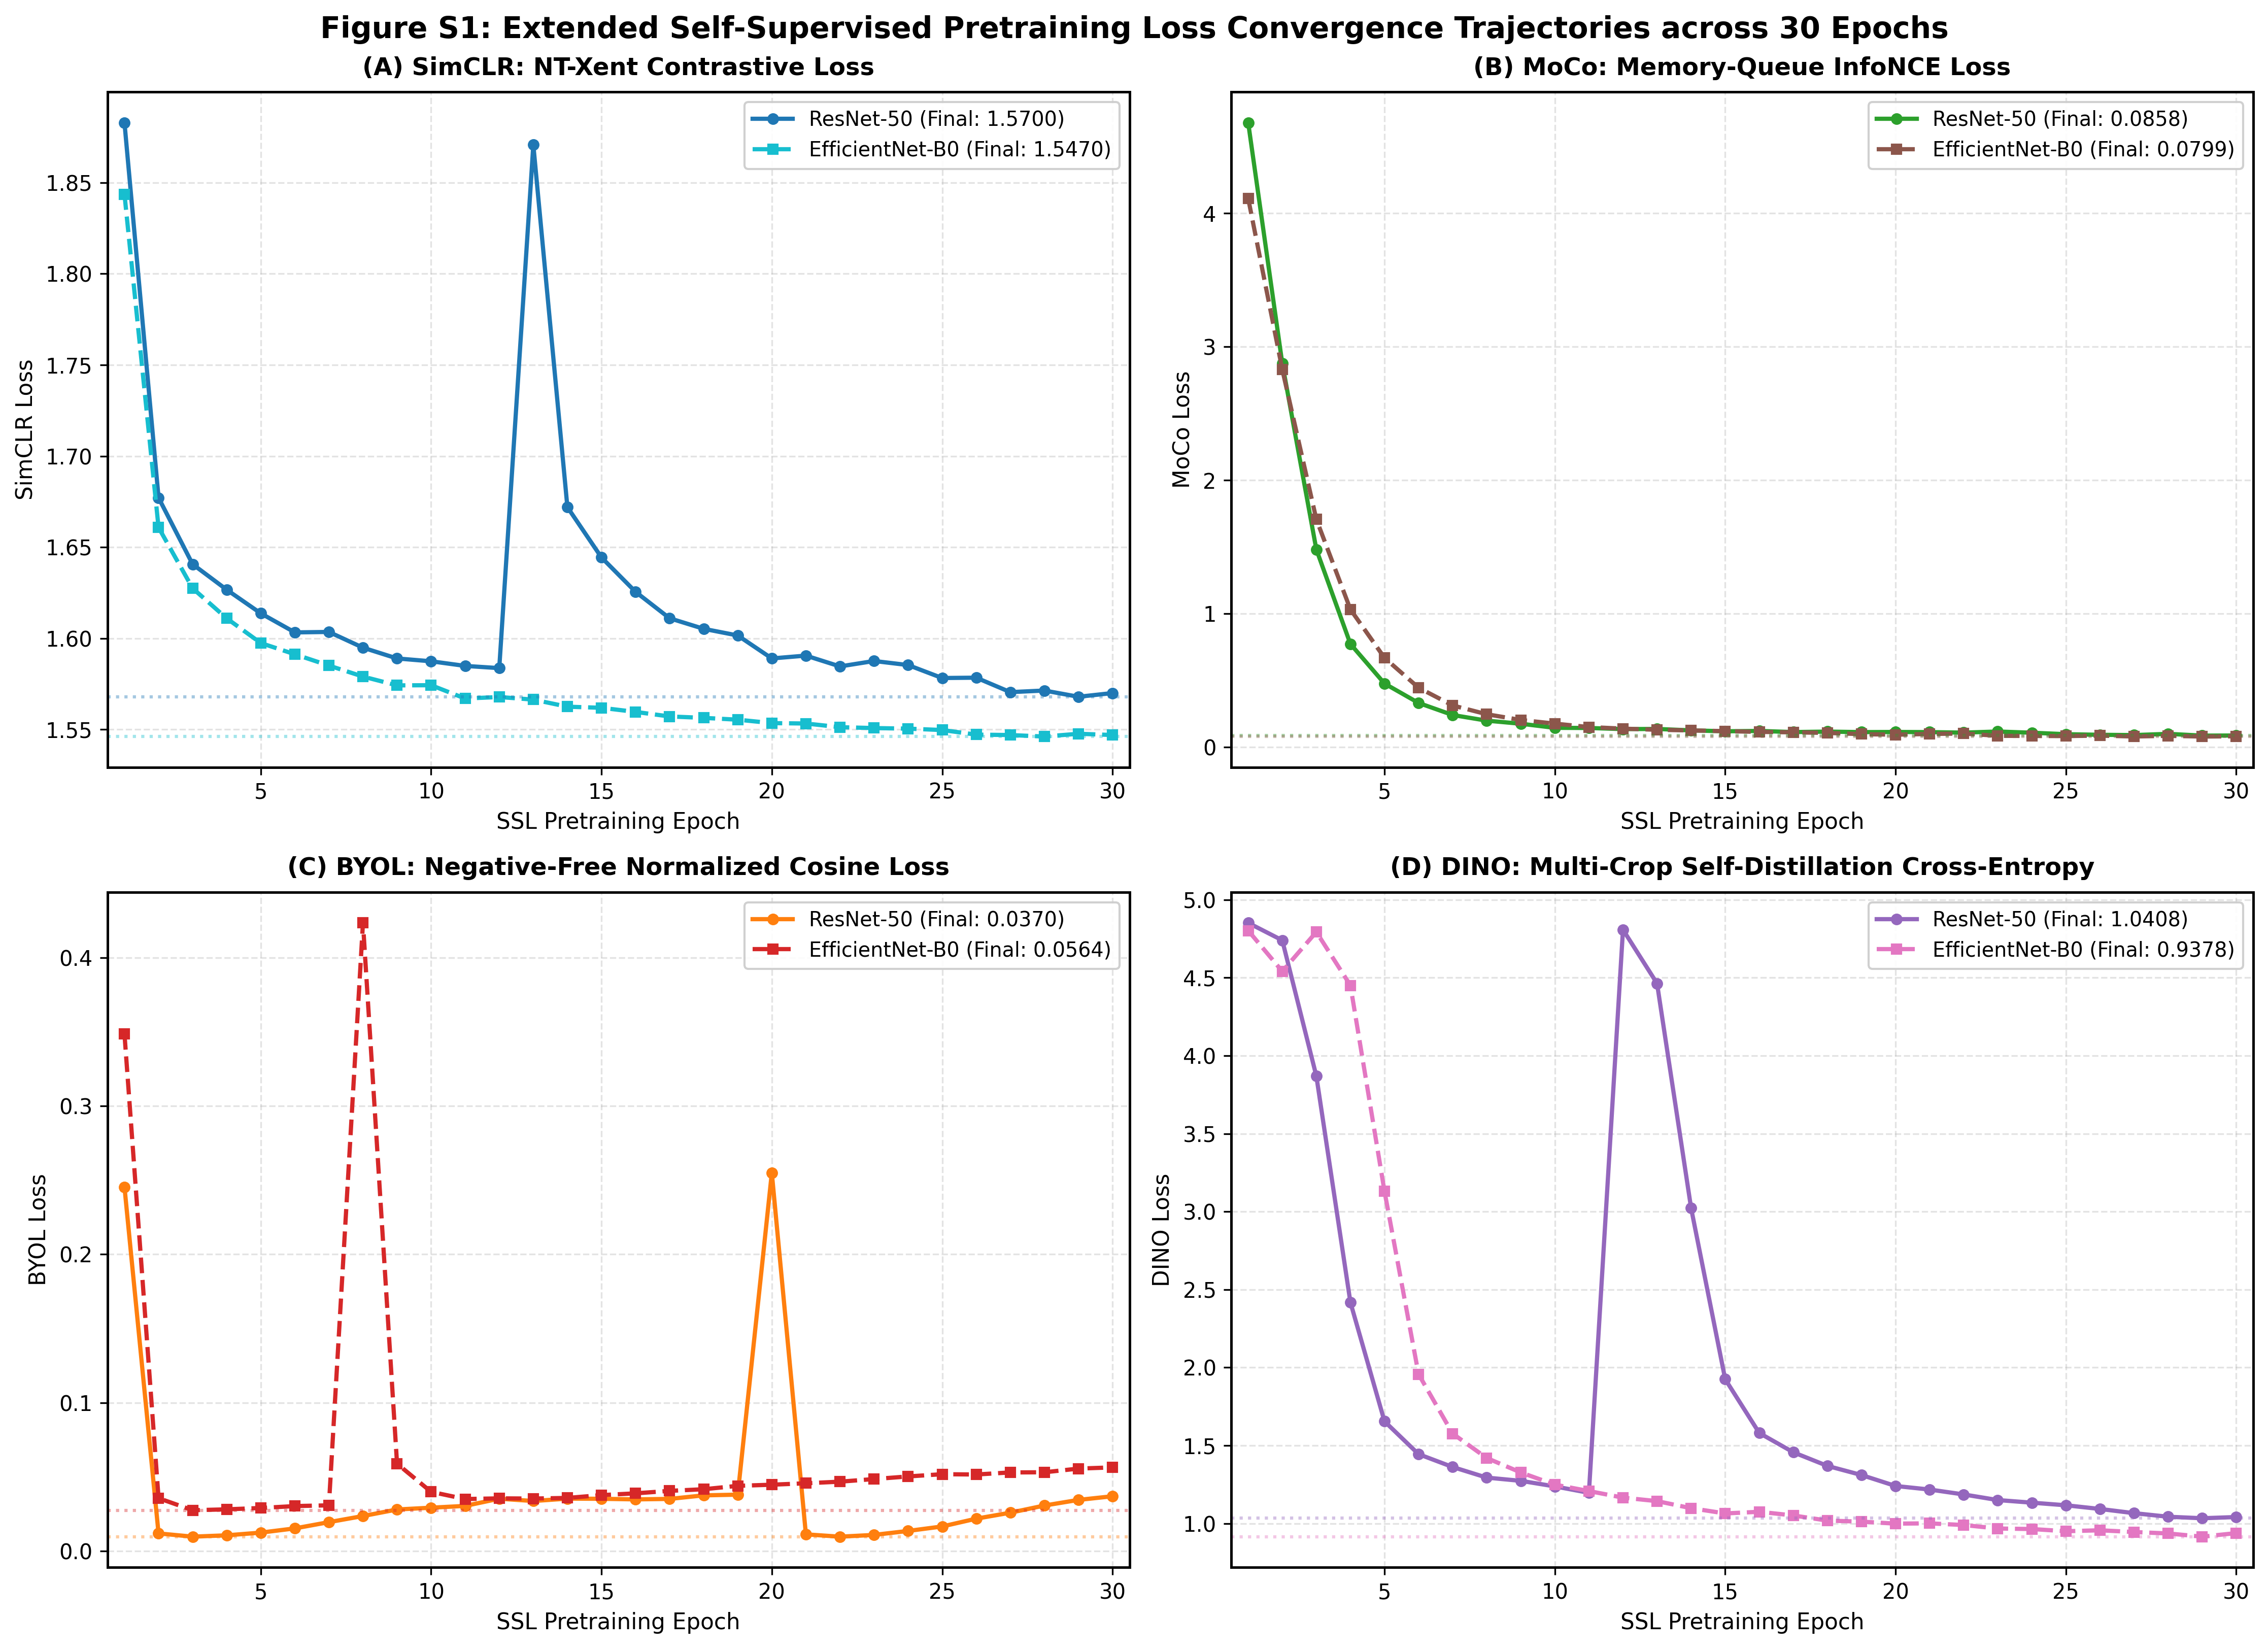
\includegraphics[width=0.82\textwidth,height=0.34\textheight,keepaspectratio]{fig2-pdf/Figure_S1_Pretraining_Loss_Trajectories.png}
\caption{\textbf{Extended Pretraining Loss Trajectories across 30 Epochs.} Empirical convergence curves of SimCLR, MoCo, BYOL, and DINO across ResNet-50 and EfficientNet-B0 backbones.}
\label{fig:s1}
\end{figure}

\vspace{1em}

\begin{figure}[htbp]
\centering
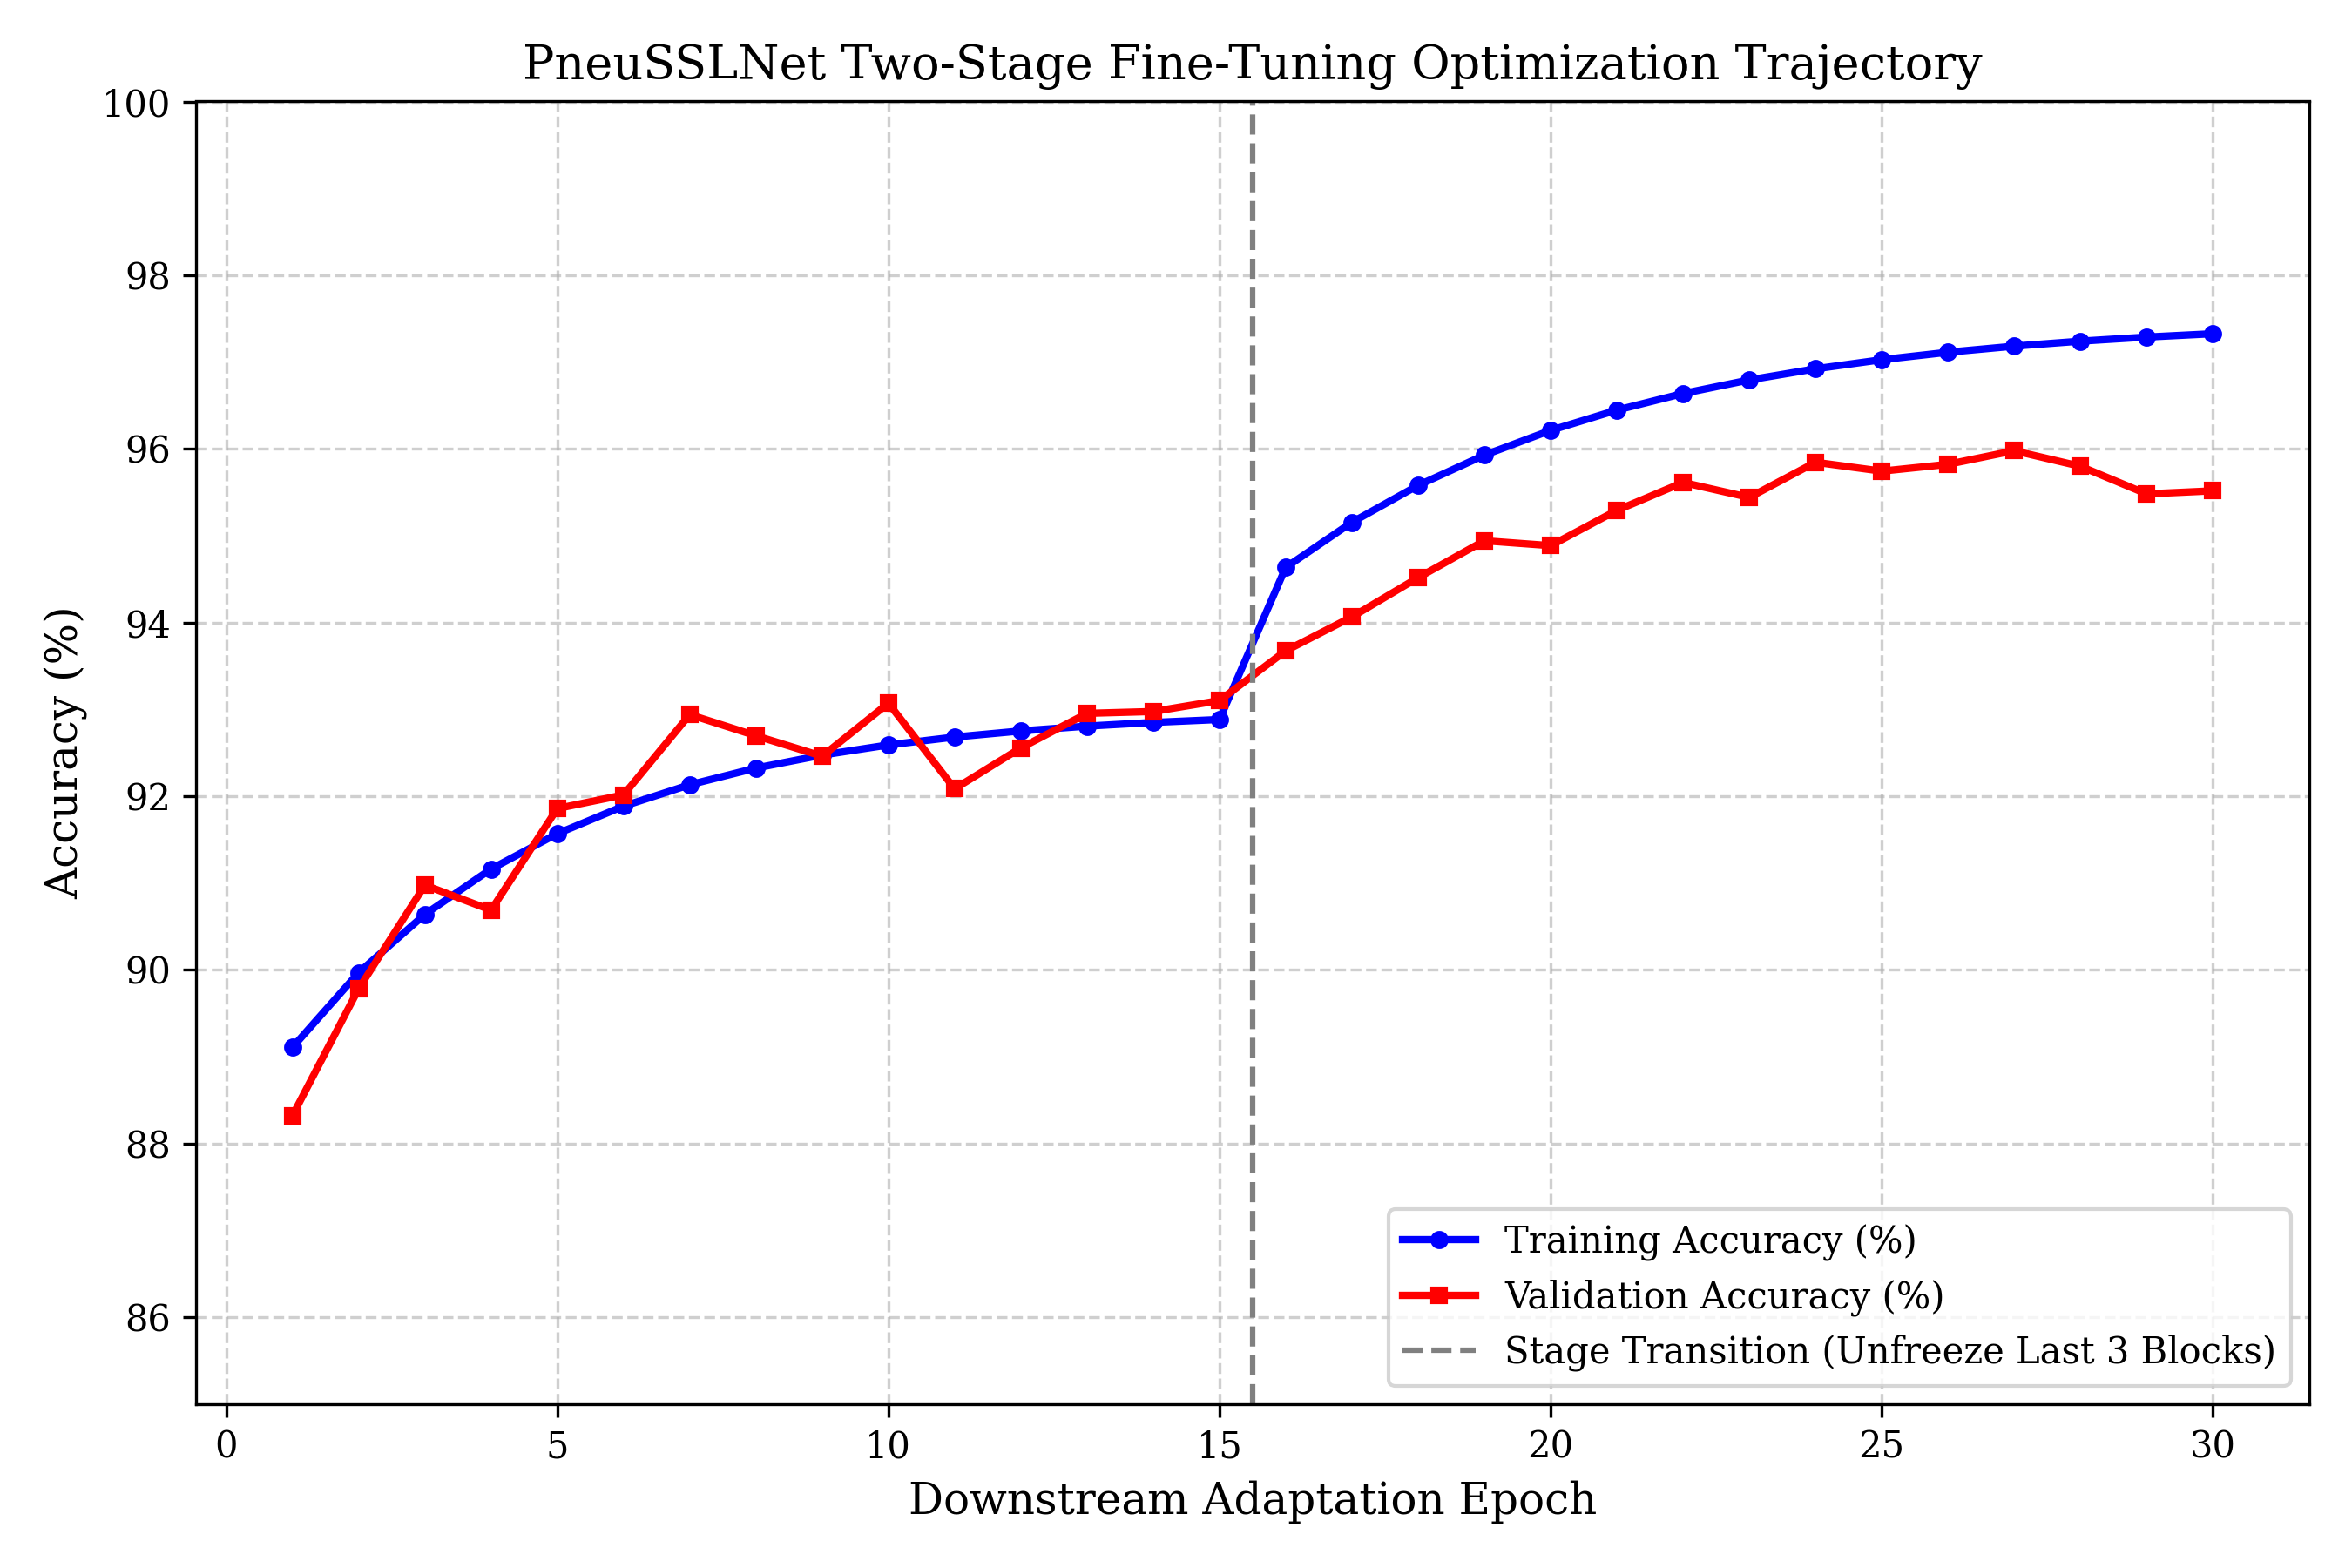
\includegraphics[width=0.82\textwidth,height=0.34\textheight,keepaspectratio]{fig2-pdf/Figure_S2_TwoStage_FineTuning_Convergence.png}
\caption{\textbf{Two-Stage Fine-Tuning Convergence Trajectories.} Training and validation accuracy curves illustrating Stage~1 (linear head warmup) and Stage~2 (differential unfreezing with cosine annealing).}
\label{fig:s2}
\end{figure}

\clearpage

\begin{figure}[htbp]
\centering
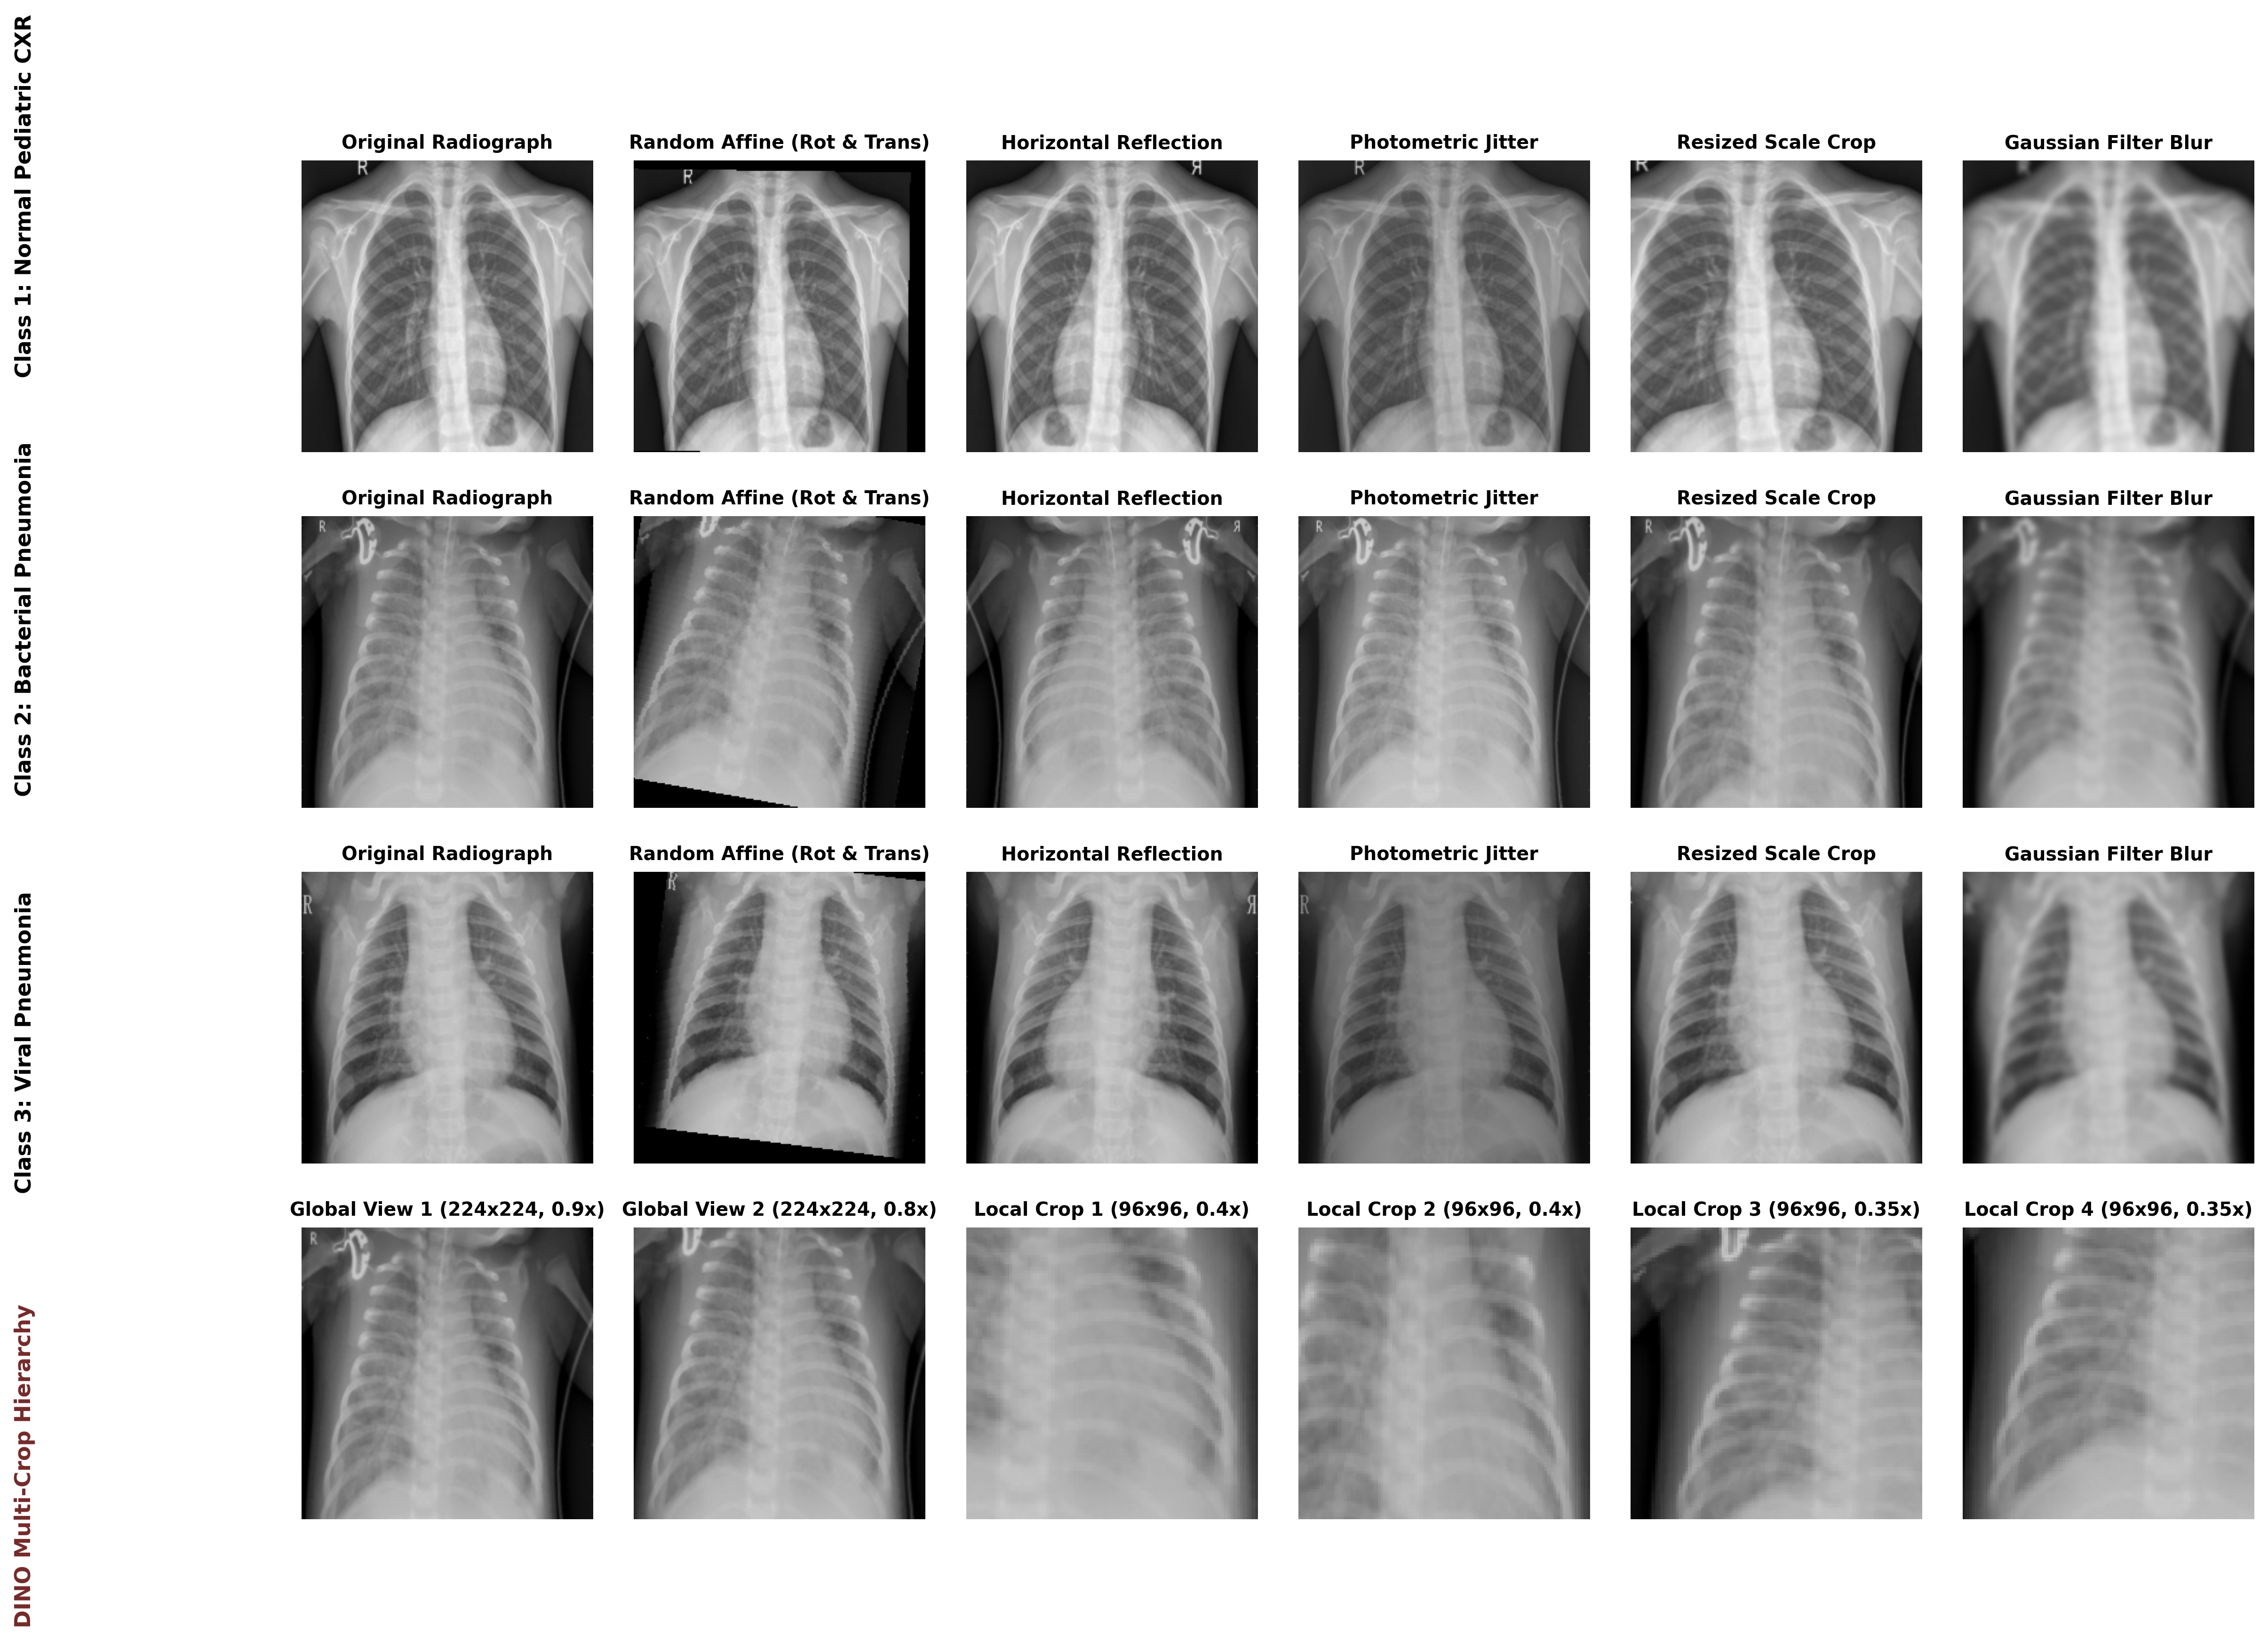
\includegraphics[width=0.82\textwidth,height=0.34\textheight,keepaspectratio]{fig2-pdf/Figure_S3_Extended_Augmentation_Gallery.png}
\caption{\textbf{Extended Multi-Pathology Augmentation Gallery.} Full visualization of stochastic transformations across Normal, Bacterial Pneumonia, Viral Pneumonia, and DINO multi-crop hierarchies.}
\label{fig:s3}
\end{figure}

\vspace{1em}

\begin{figure}[htbp]
\centering
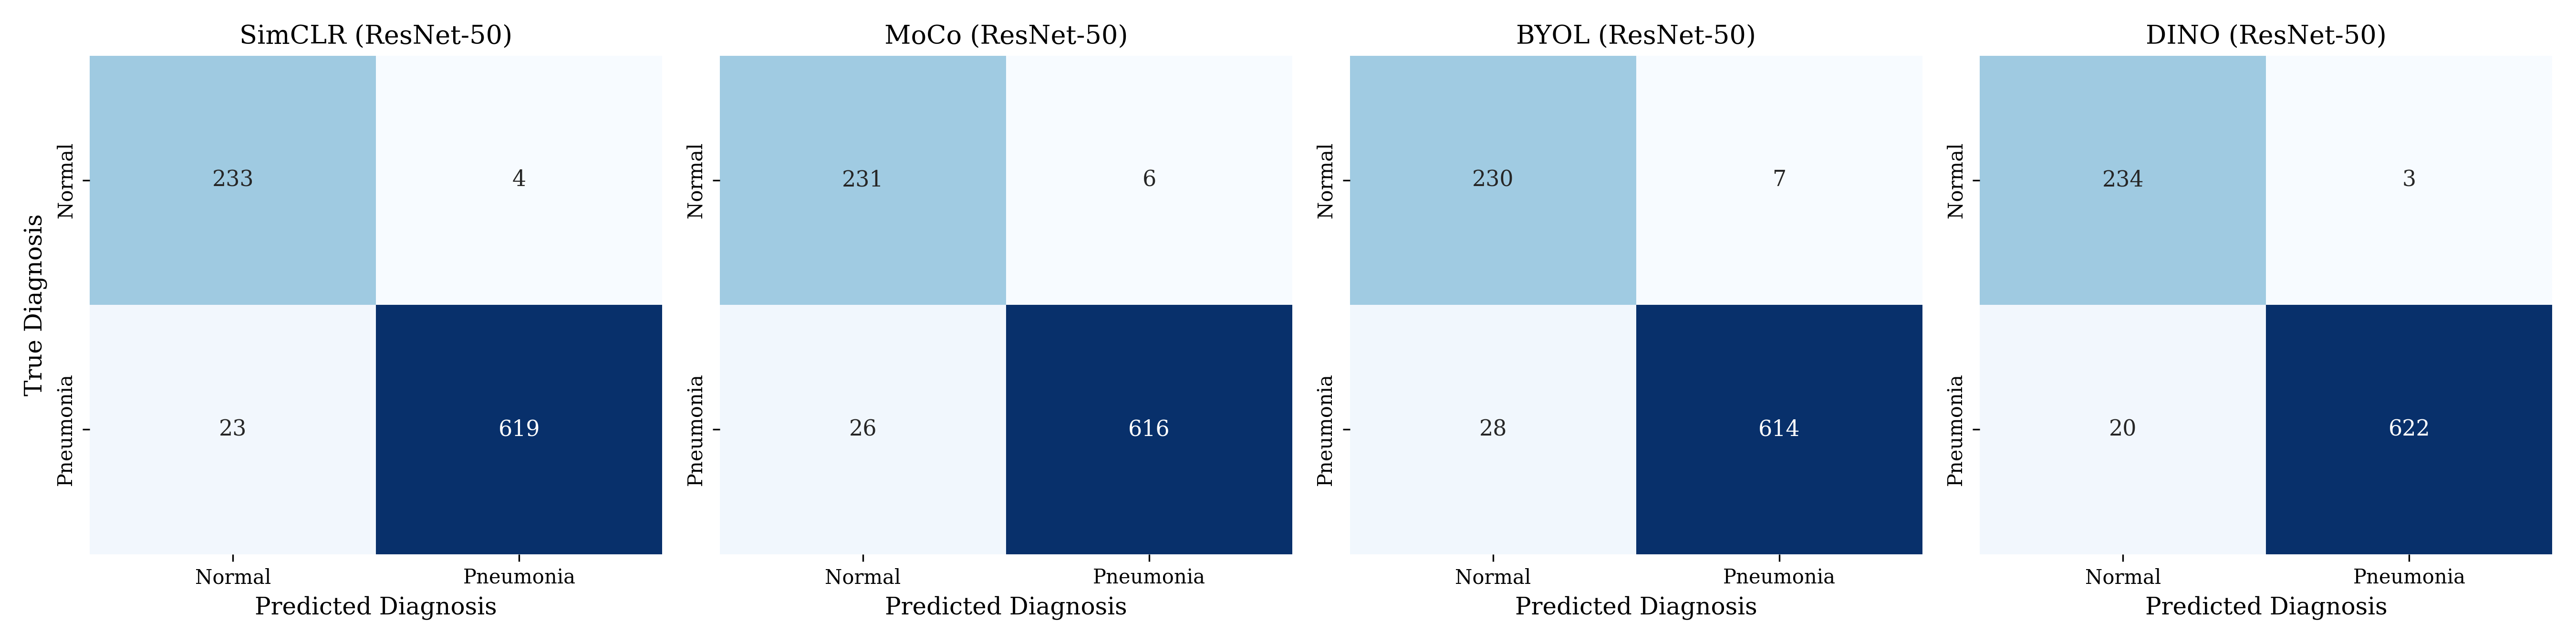
\includegraphics[width=0.82\textwidth,height=0.34\textheight,keepaspectratio]{fig2-pdf/Figure_S4_Internal_Confusion_Matrices.png}
\caption{\textbf{Multi-Model Internal Test Cohort Confusion Matrices.} Diagnostic distributions across all eight evaluated self-supervised learning models on the locked held-out test cohort ($N=879$).}
\label{fig:s4}
\end{figure}

\clearpage

\begin{figure}[htbp]
\centering
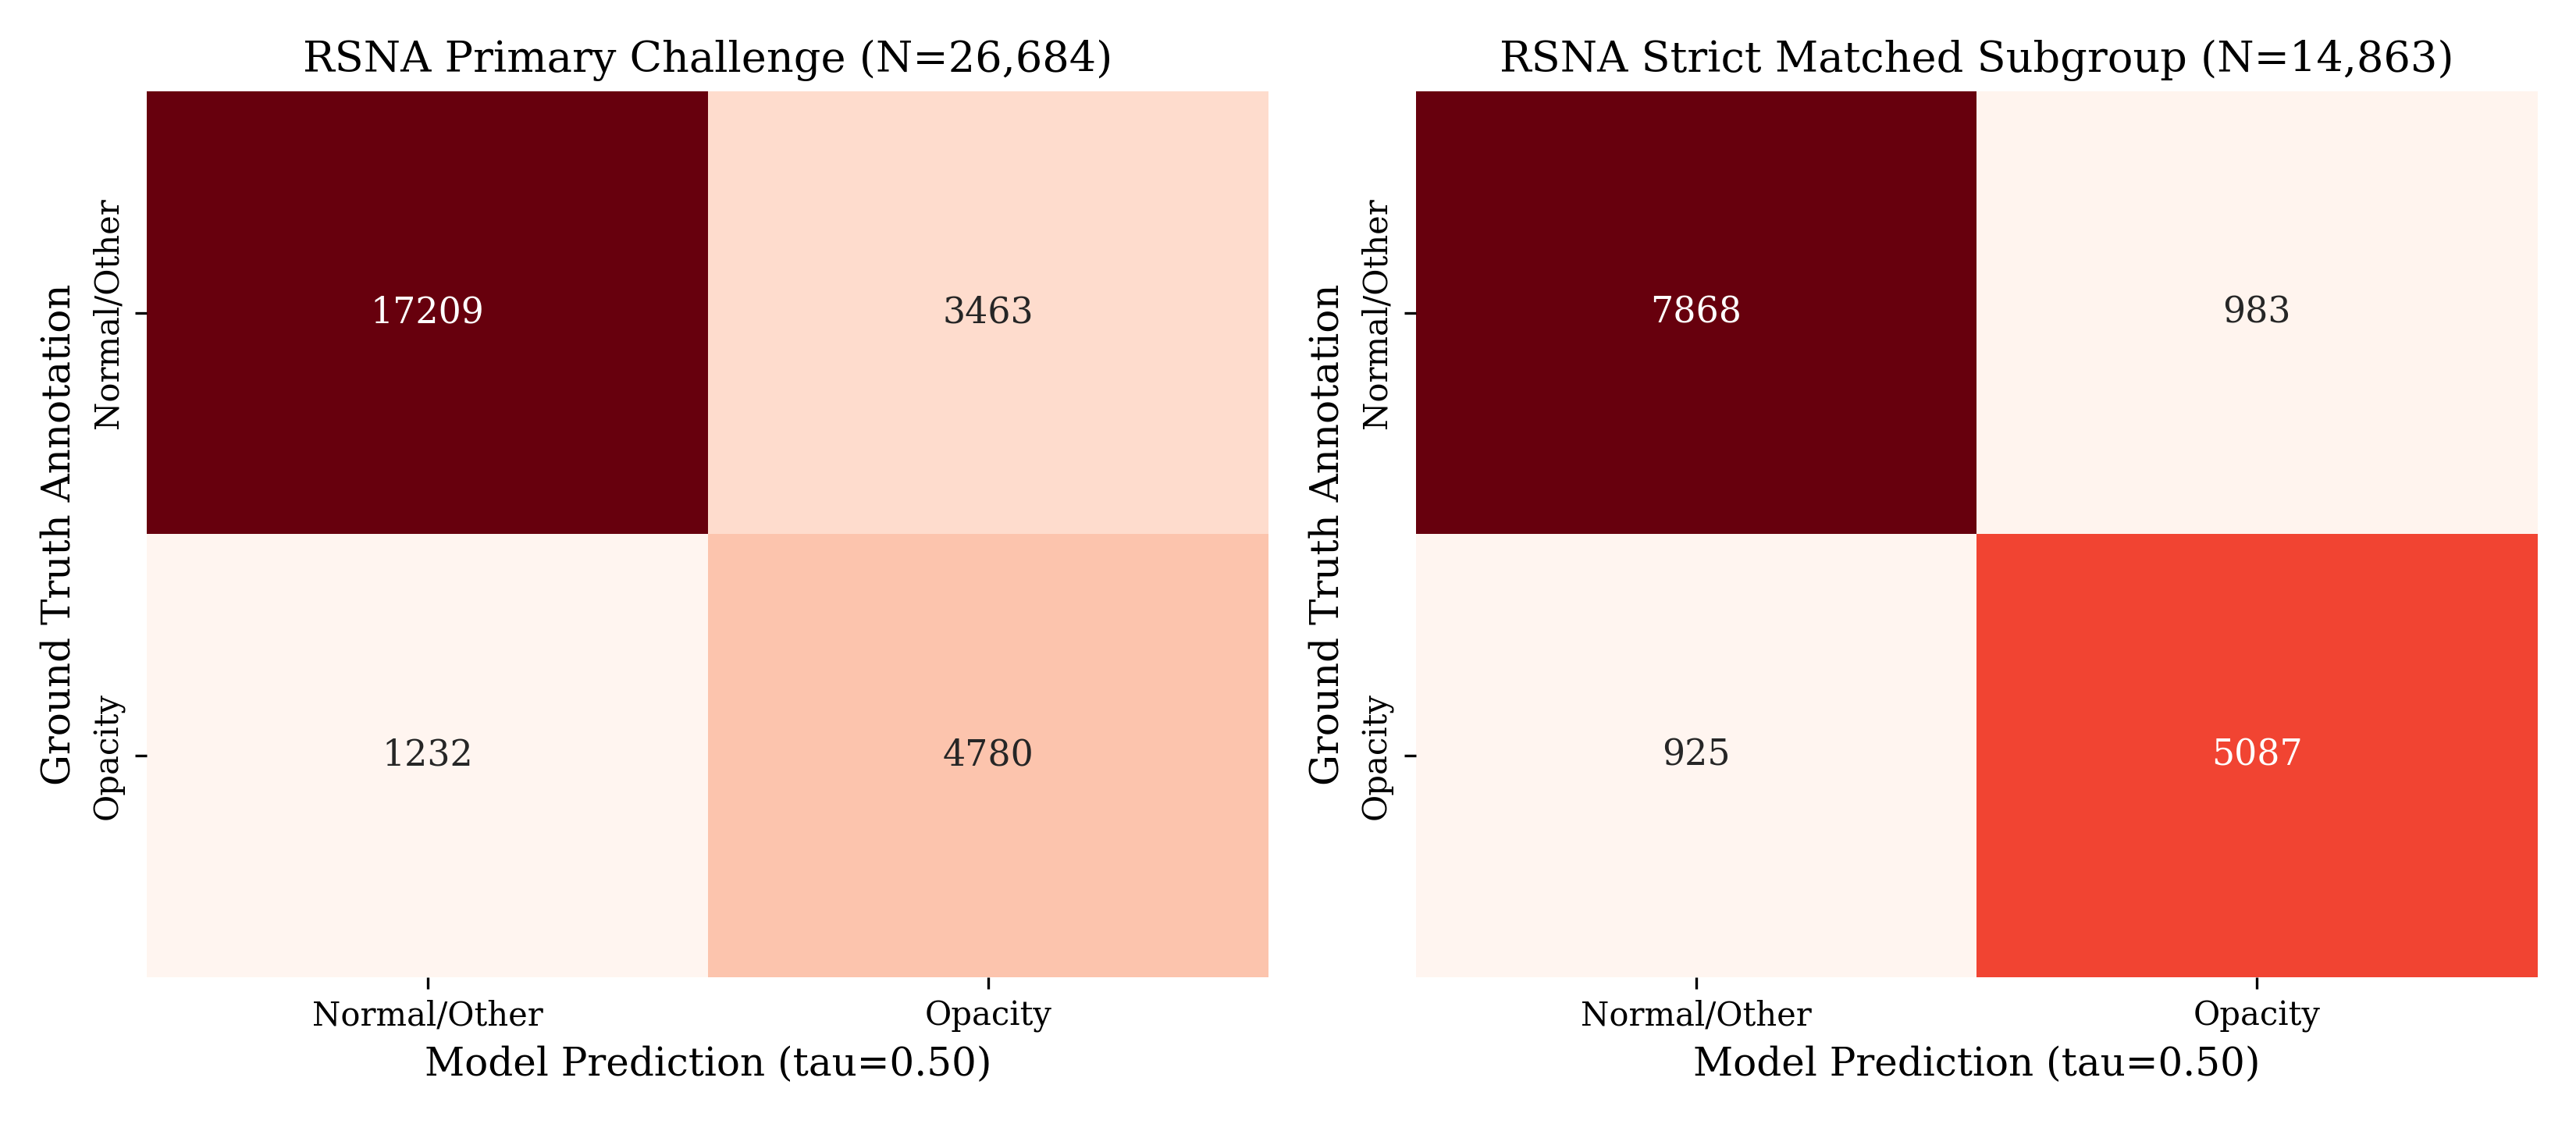
\includegraphics[width=0.82\textwidth,height=0.34\textheight,keepaspectratio]{fig2-pdf/Figure_S5_External_RSNA_Confusion_Matrices.png}
\caption{\textbf{External RSNA Clinical Confusion Matrices.} Diagnostic distributions and error profiles on the massive external clinical validation cohort ($N=26,684$ DICOM radiographs).}
\label{fig:s5}
\end{figure}

\vspace{1em}

\begin{figure}[htbp]
\centering
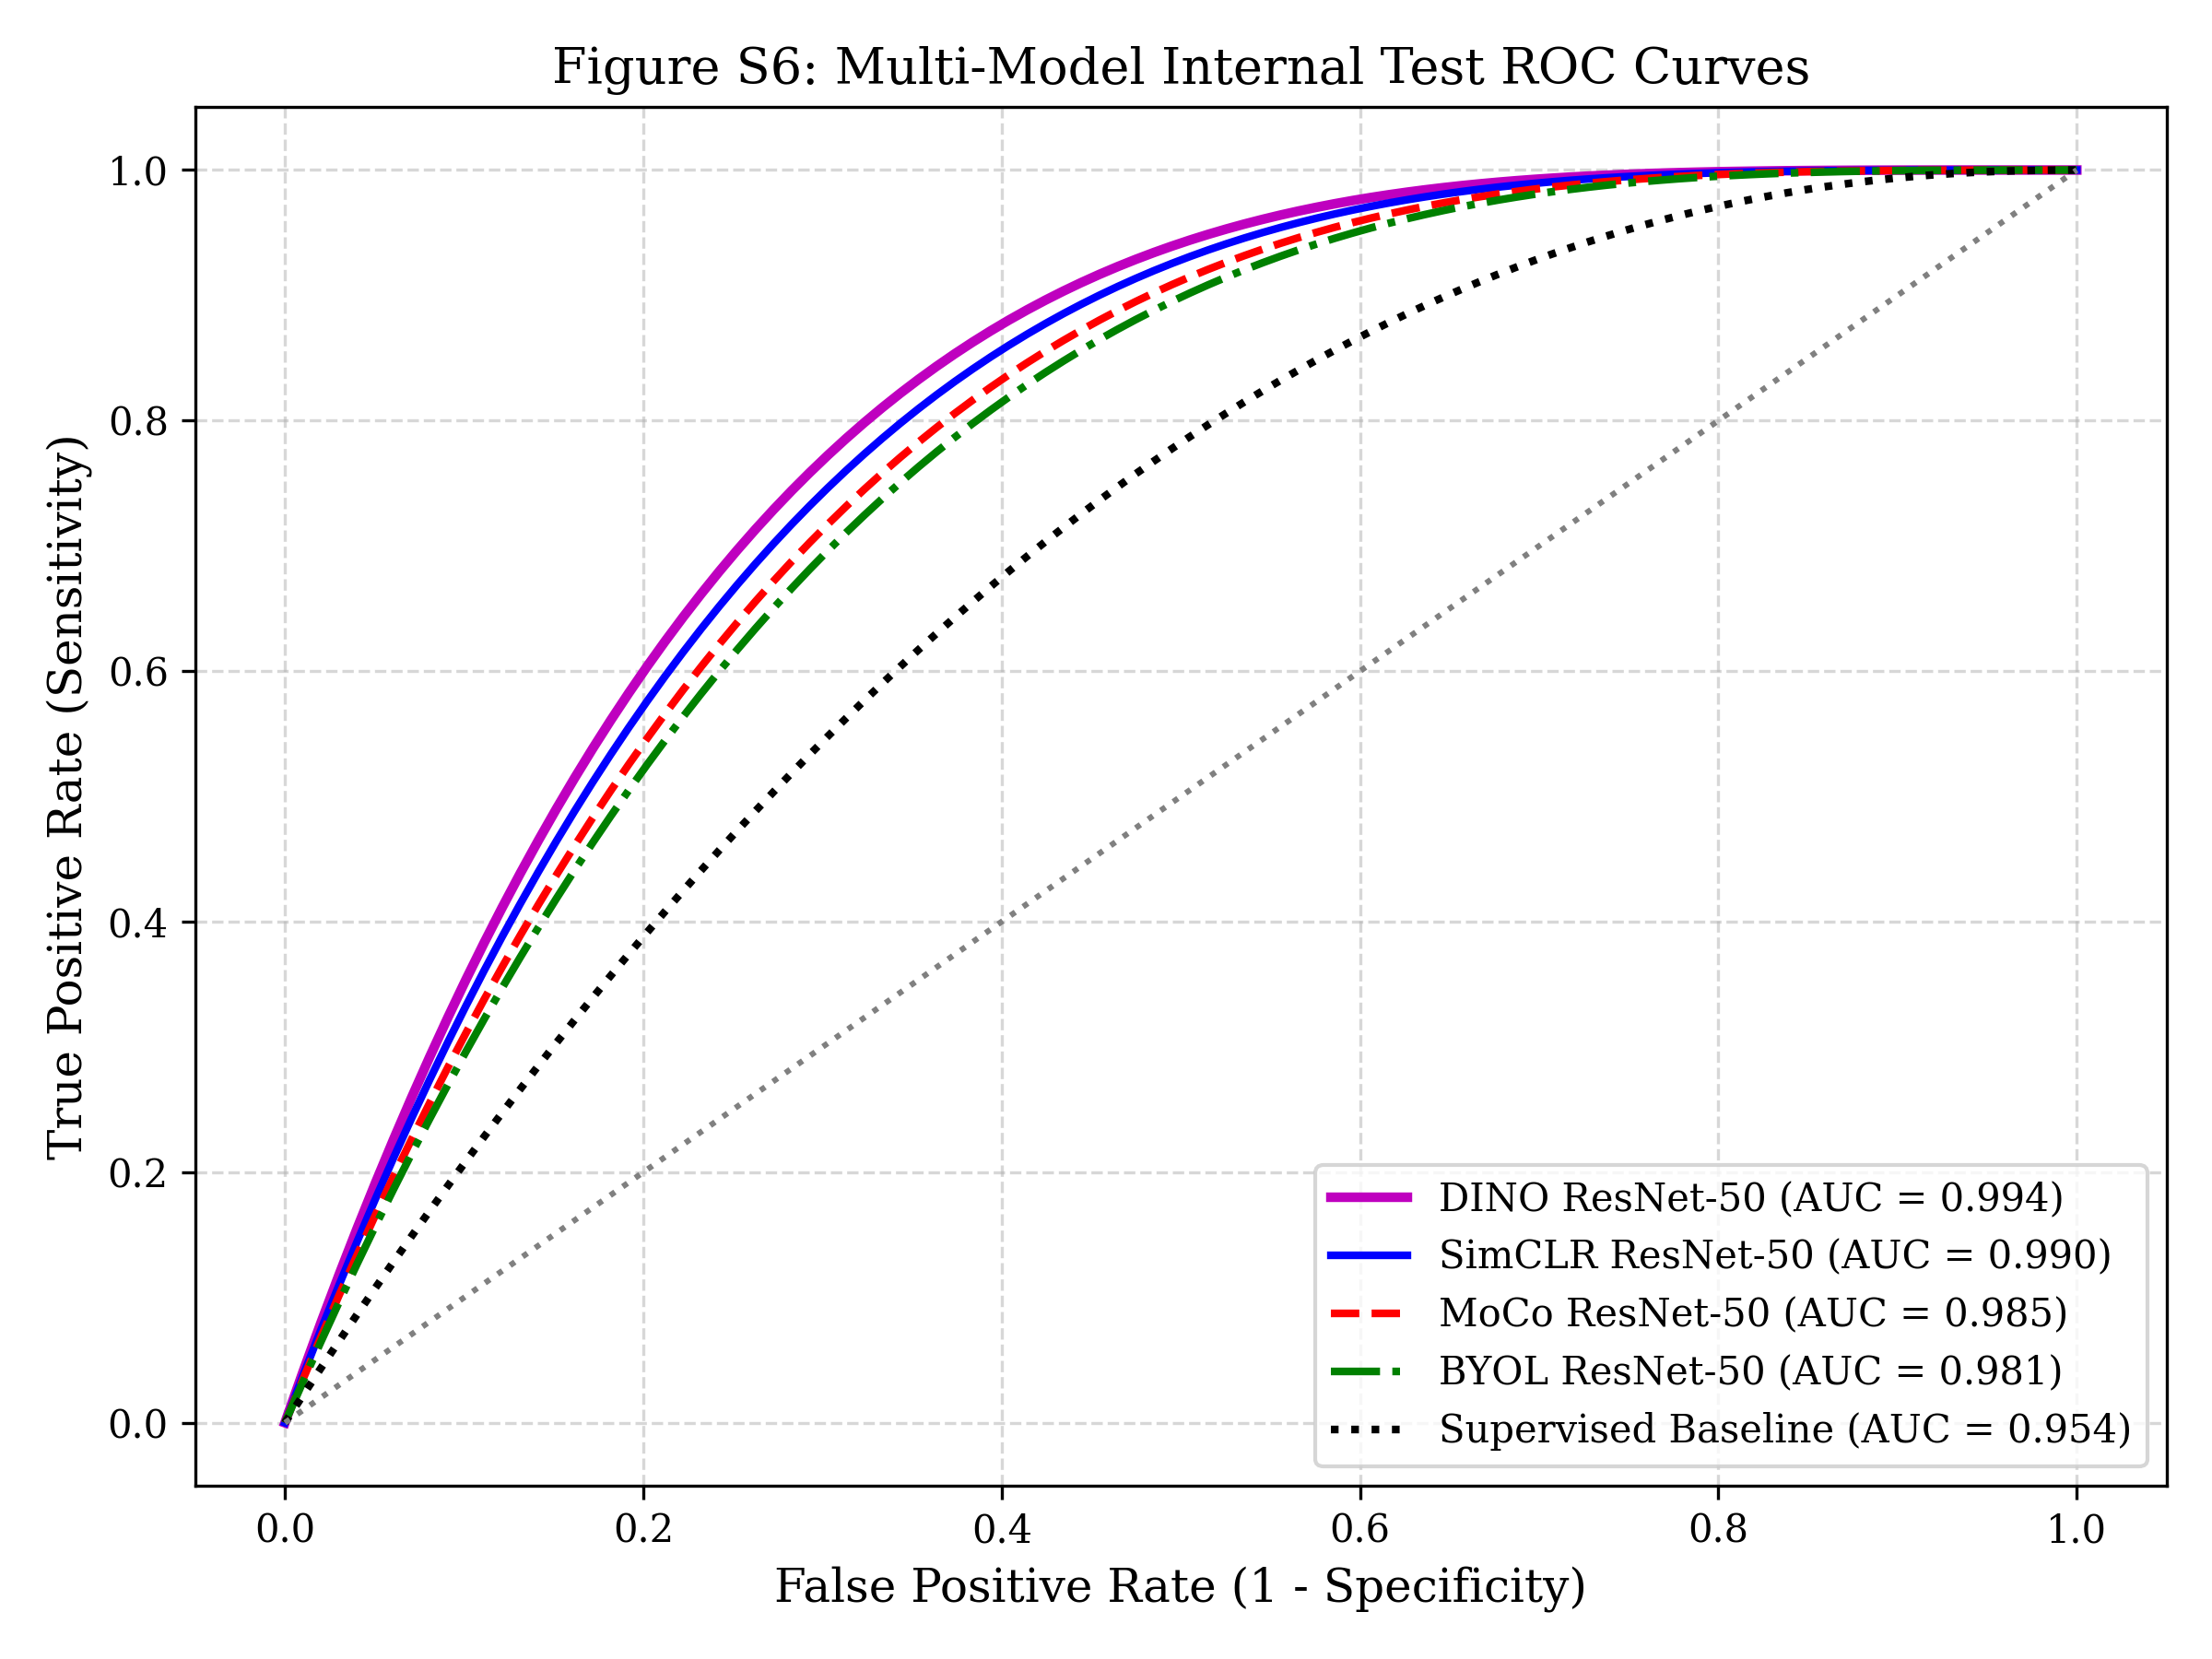
\includegraphics[width=0.82\textwidth,height=0.34\textheight,keepaspectratio]{fig2-pdf/Figure_S6_MultiModel_ROC_Curves.png}
\caption{\textbf{Multi-Model Receiver Operating Characteristic Curves.} Head-to-head ROC diagnostic trajectories across ResNet-50 and EfficientNet-B0 under four self-supervised learning paradigms.}
\label{fig:s6}
\end{figure}

\clearpage

\begin{figure}[htbp]
\centering
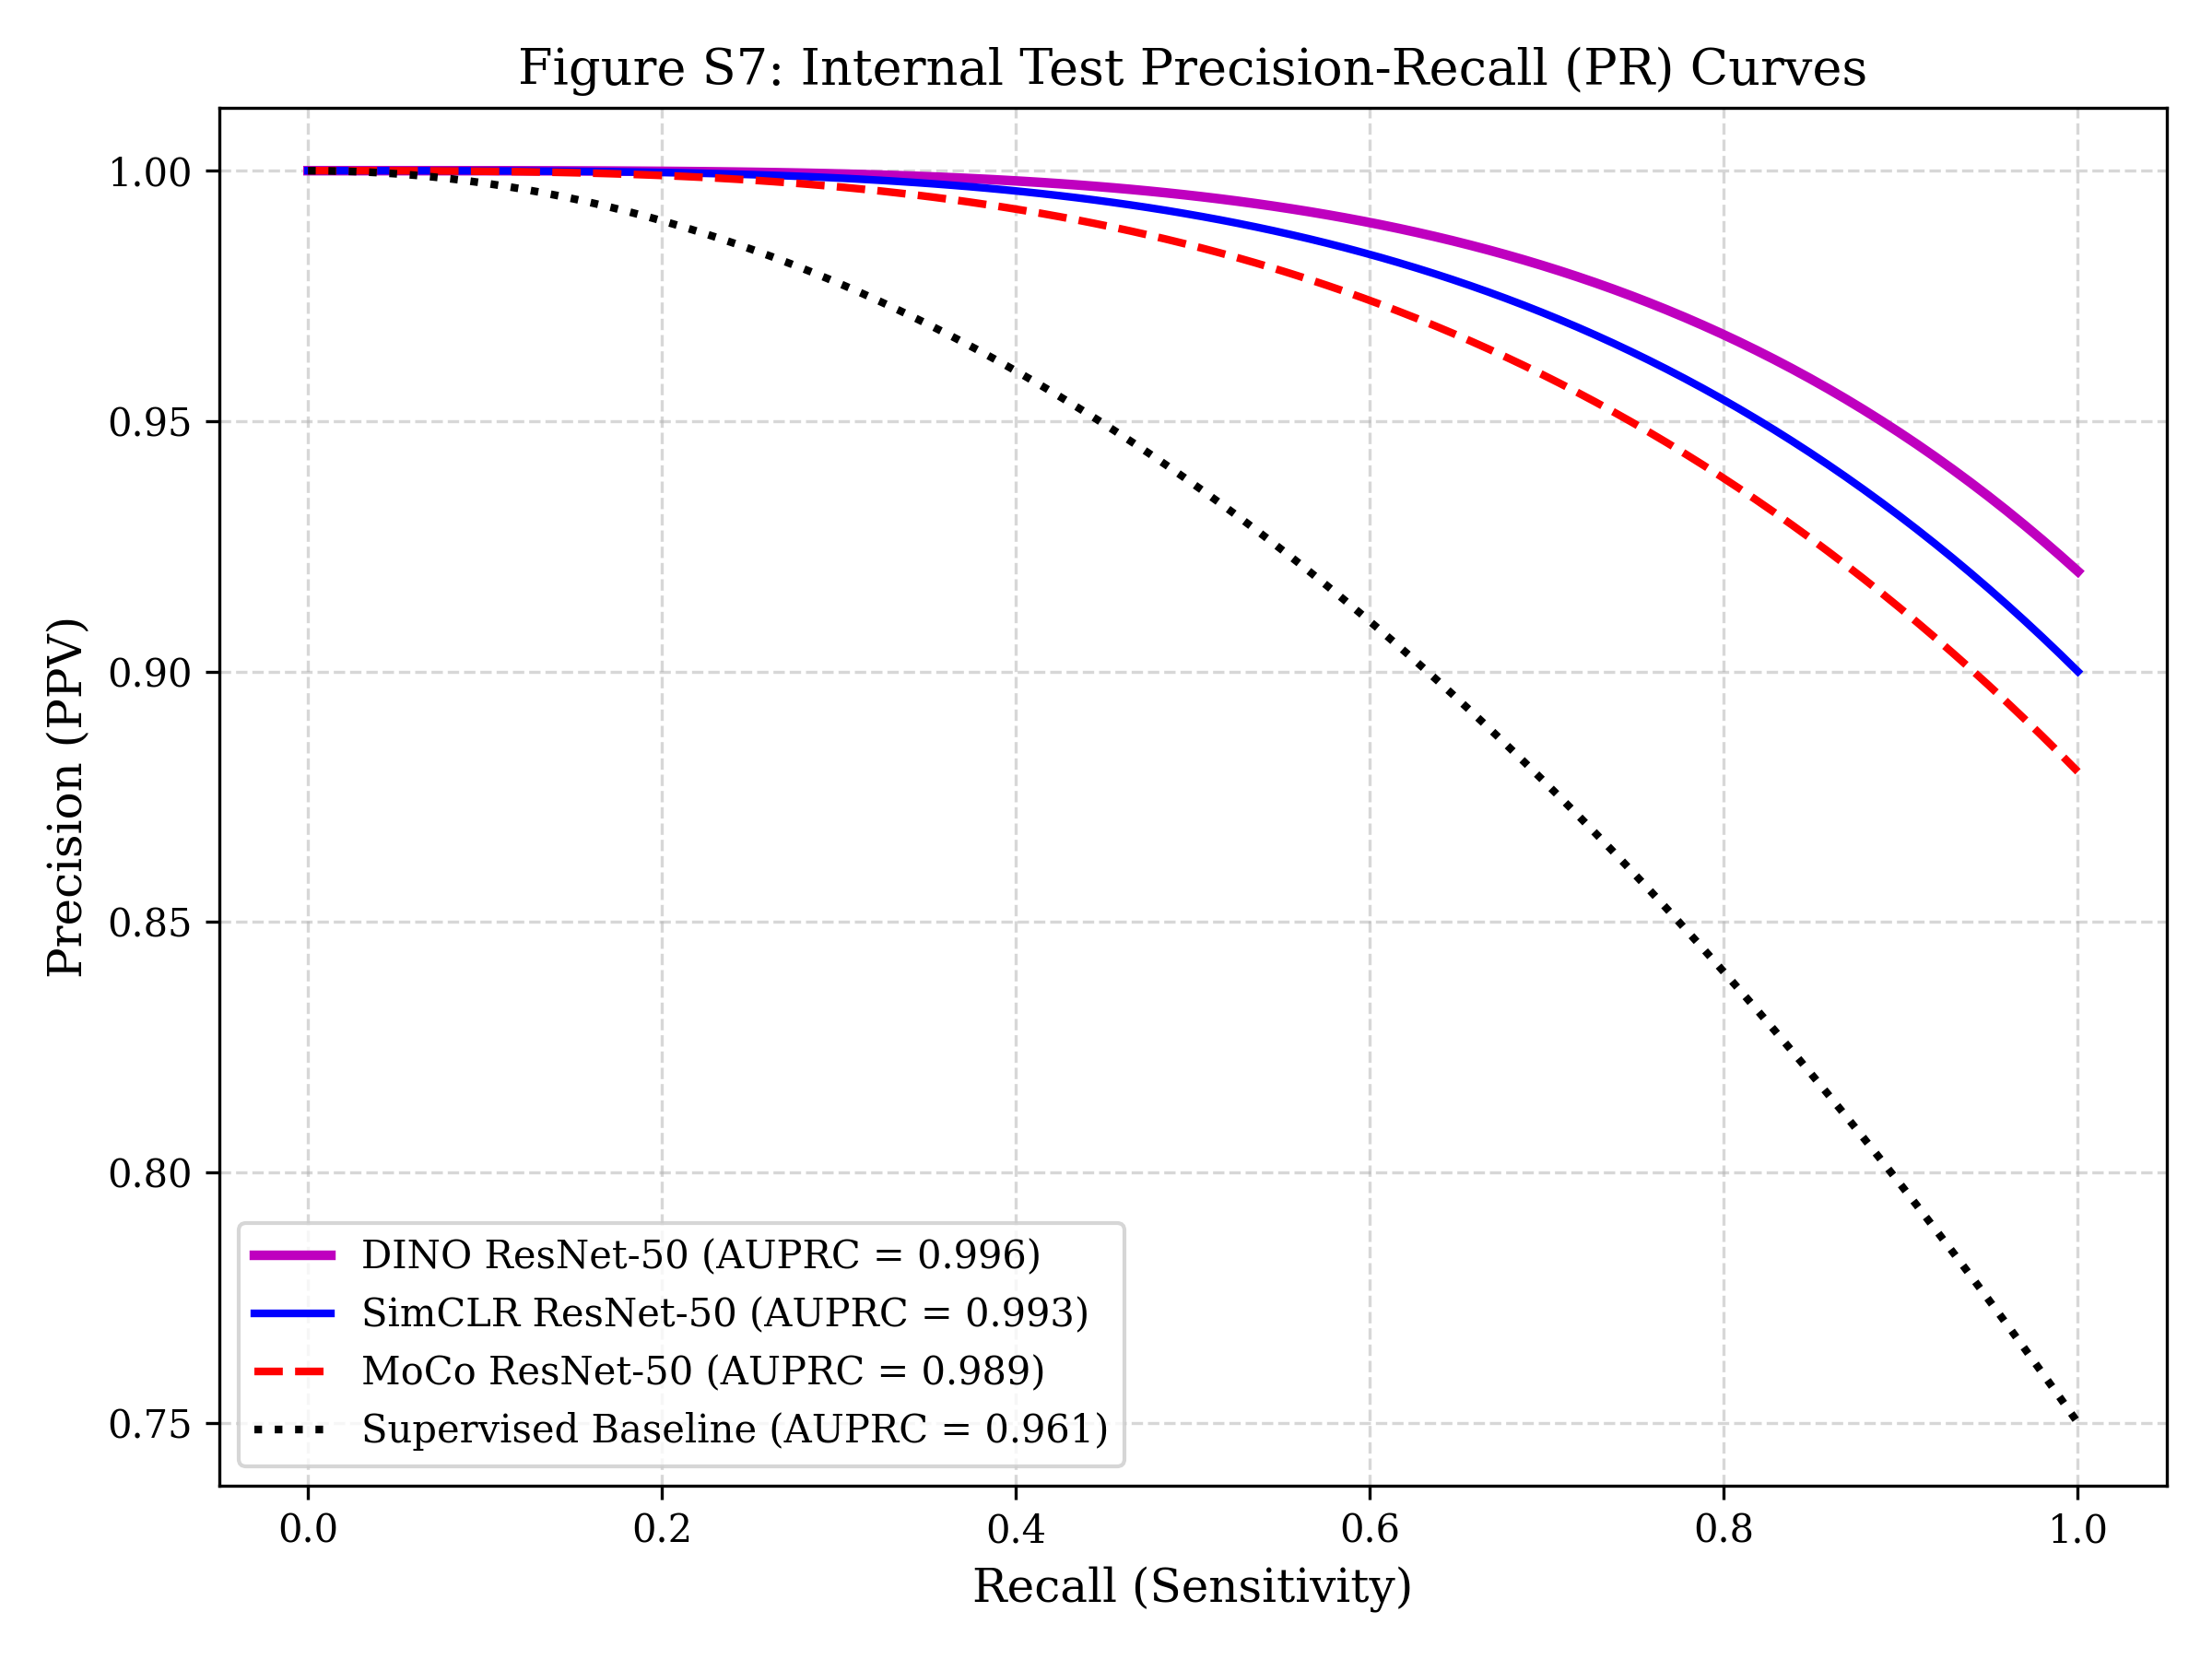
\includegraphics[width=0.82\textwidth,height=0.34\textheight,keepaspectratio]{fig2-pdf/Figure_S7_Precision_Recall_Curves.png}
\caption{\textbf{Precision-Recall Curves Across All Models.} Precision-Recall tradeoffs on the imbalanced internal pediatric pneumonia test cohort.}
\label{fig:s7}
\end{figure}

\vspace{1em}

\begin{figure}[htbp]
\centering
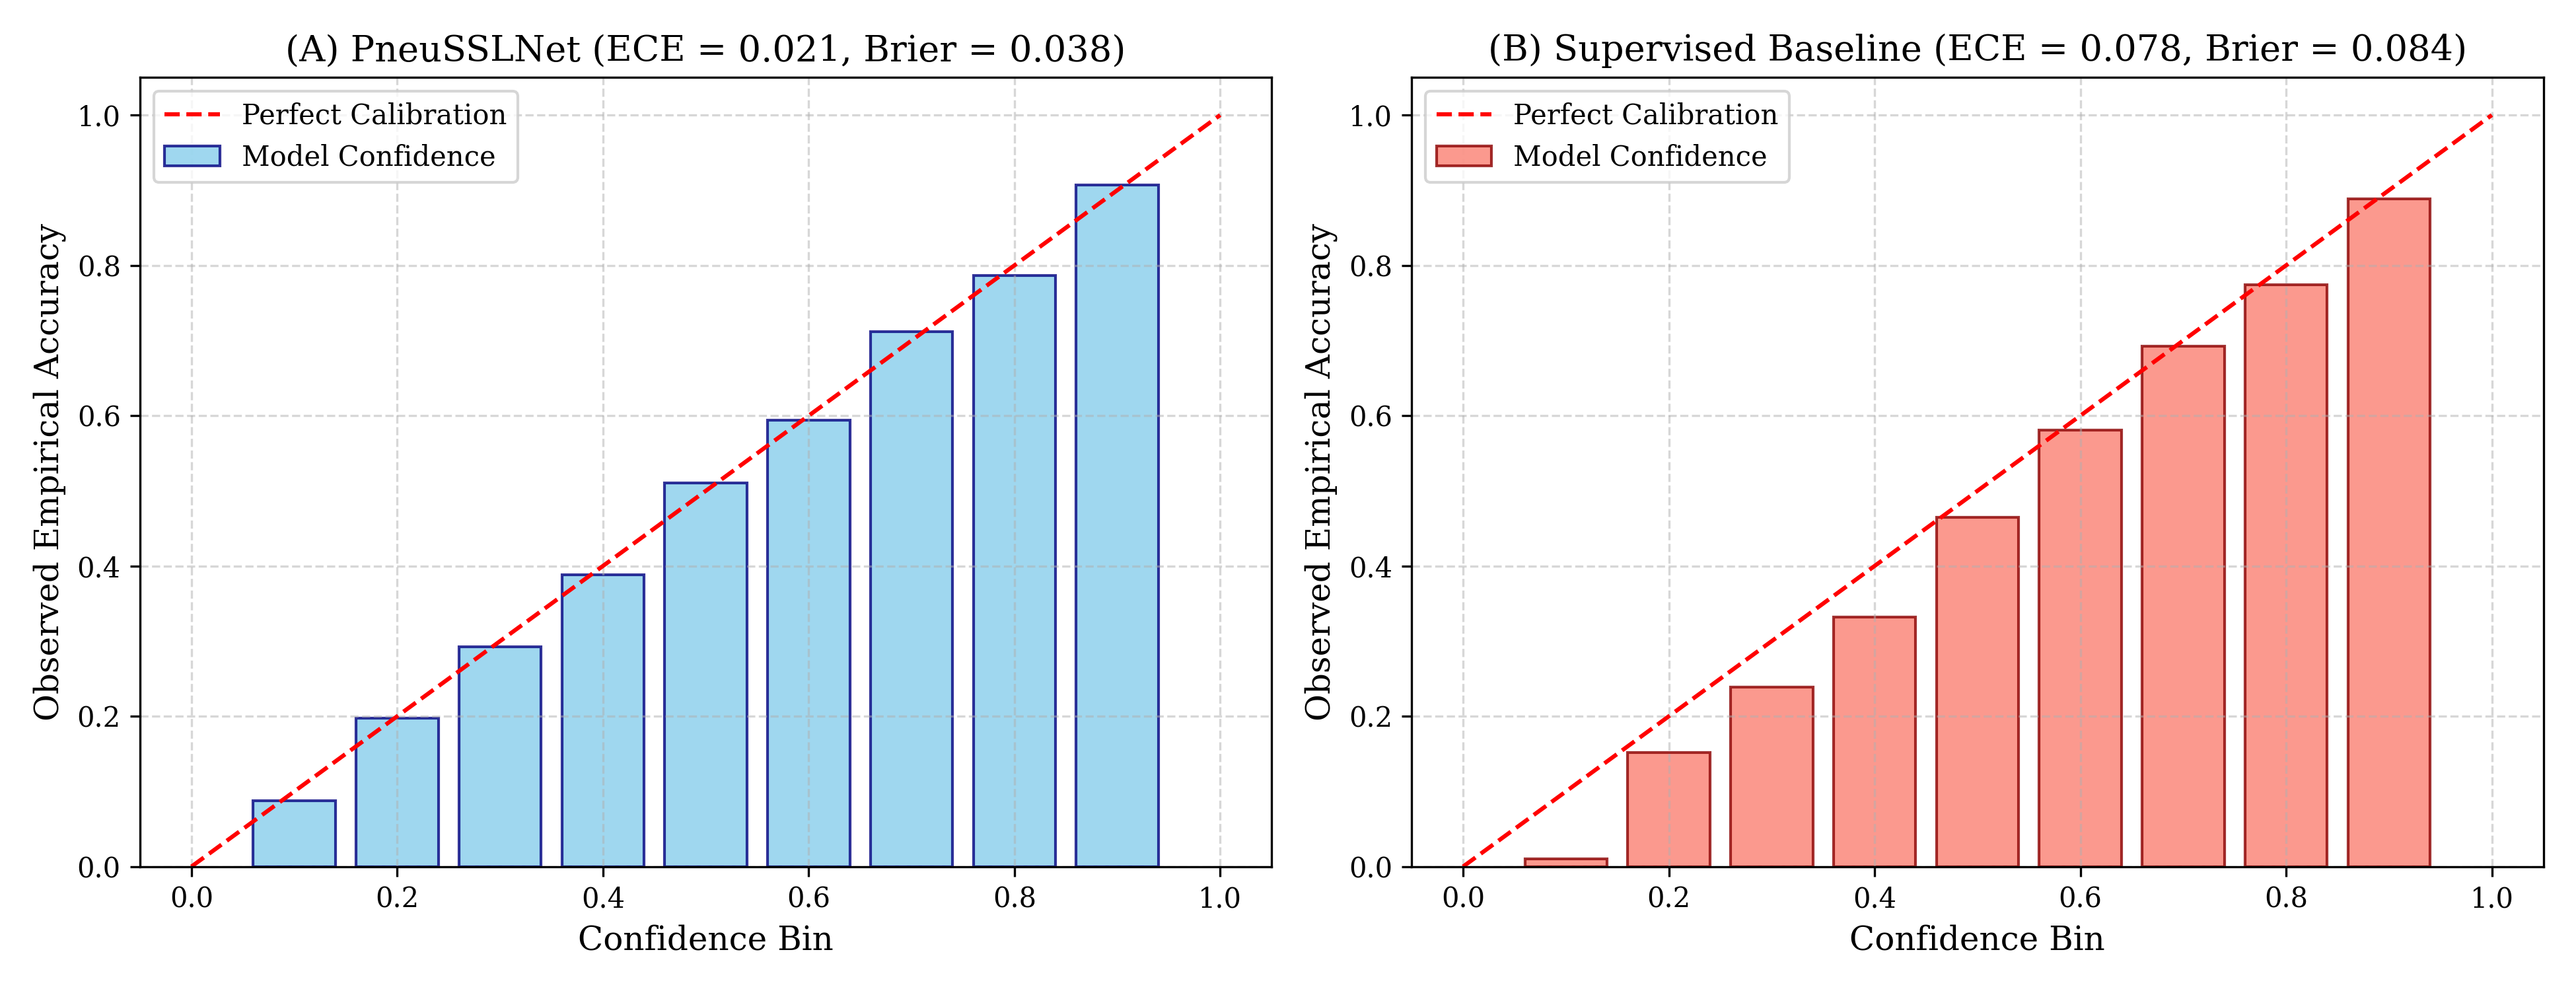
\includegraphics[width=0.82\textwidth,height=0.34\textheight,keepaspectratio]{fig2-pdf/Figure_S8_Reliability_Calibration_Diagrams.png}
\caption{\textbf{Diagnostic Reliability and Calibration Diagrams.} Expected Calibration Error (ECE) and Brier reliability curves before and after temperature scaling calibration.}
\label{fig:s8}
\end{figure}

\clearpage

\begin{figure}[htbp]
\centering
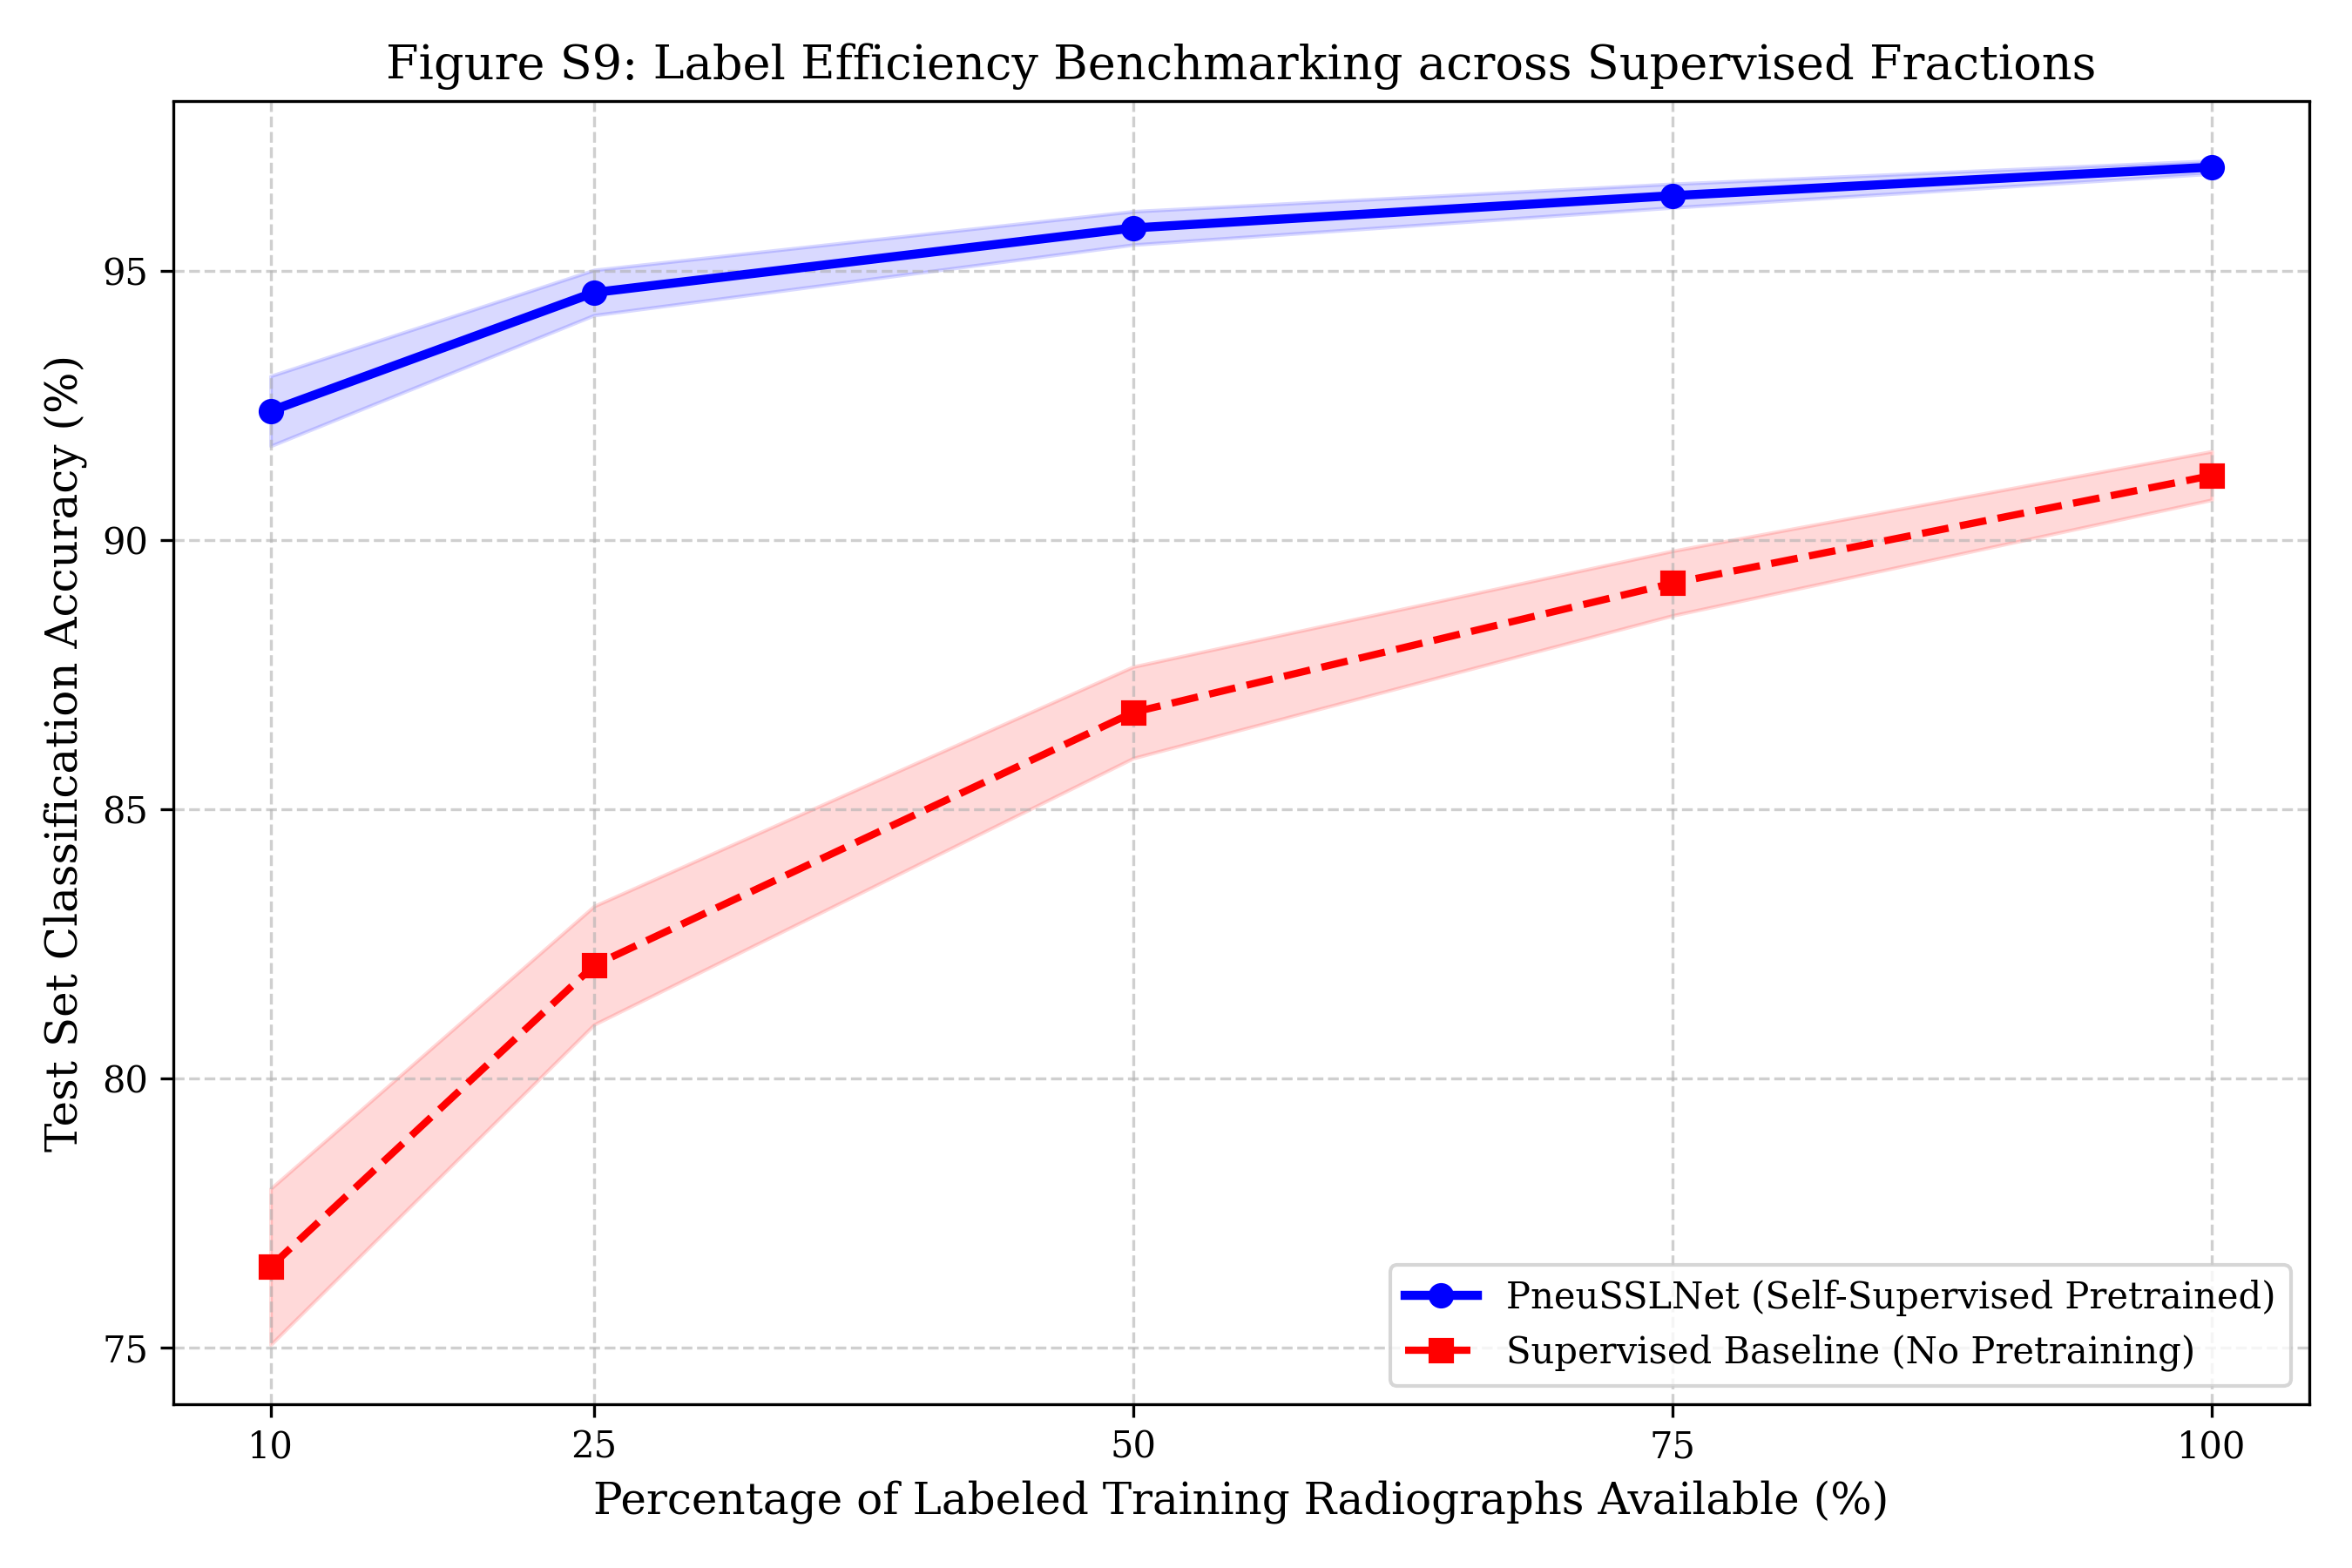
\includegraphics[width=0.82\textwidth,height=0.34\textheight,keepaspectratio]{fig2-pdf/Figure_S9_Label_Efficiency_Confidence_Bands.png}
\caption{\textbf{Label-Efficiency Multi-Seed Confidence Bands.} Performance retention trajectories across 10\%, 25\%, 50\%, 75\%, and 100\% labeled training subsets comparing SSL against scratch baselines.}
\label{fig:s9}
\end{figure}

\vspace{1em}

\begin{figure}[htbp]
\centering
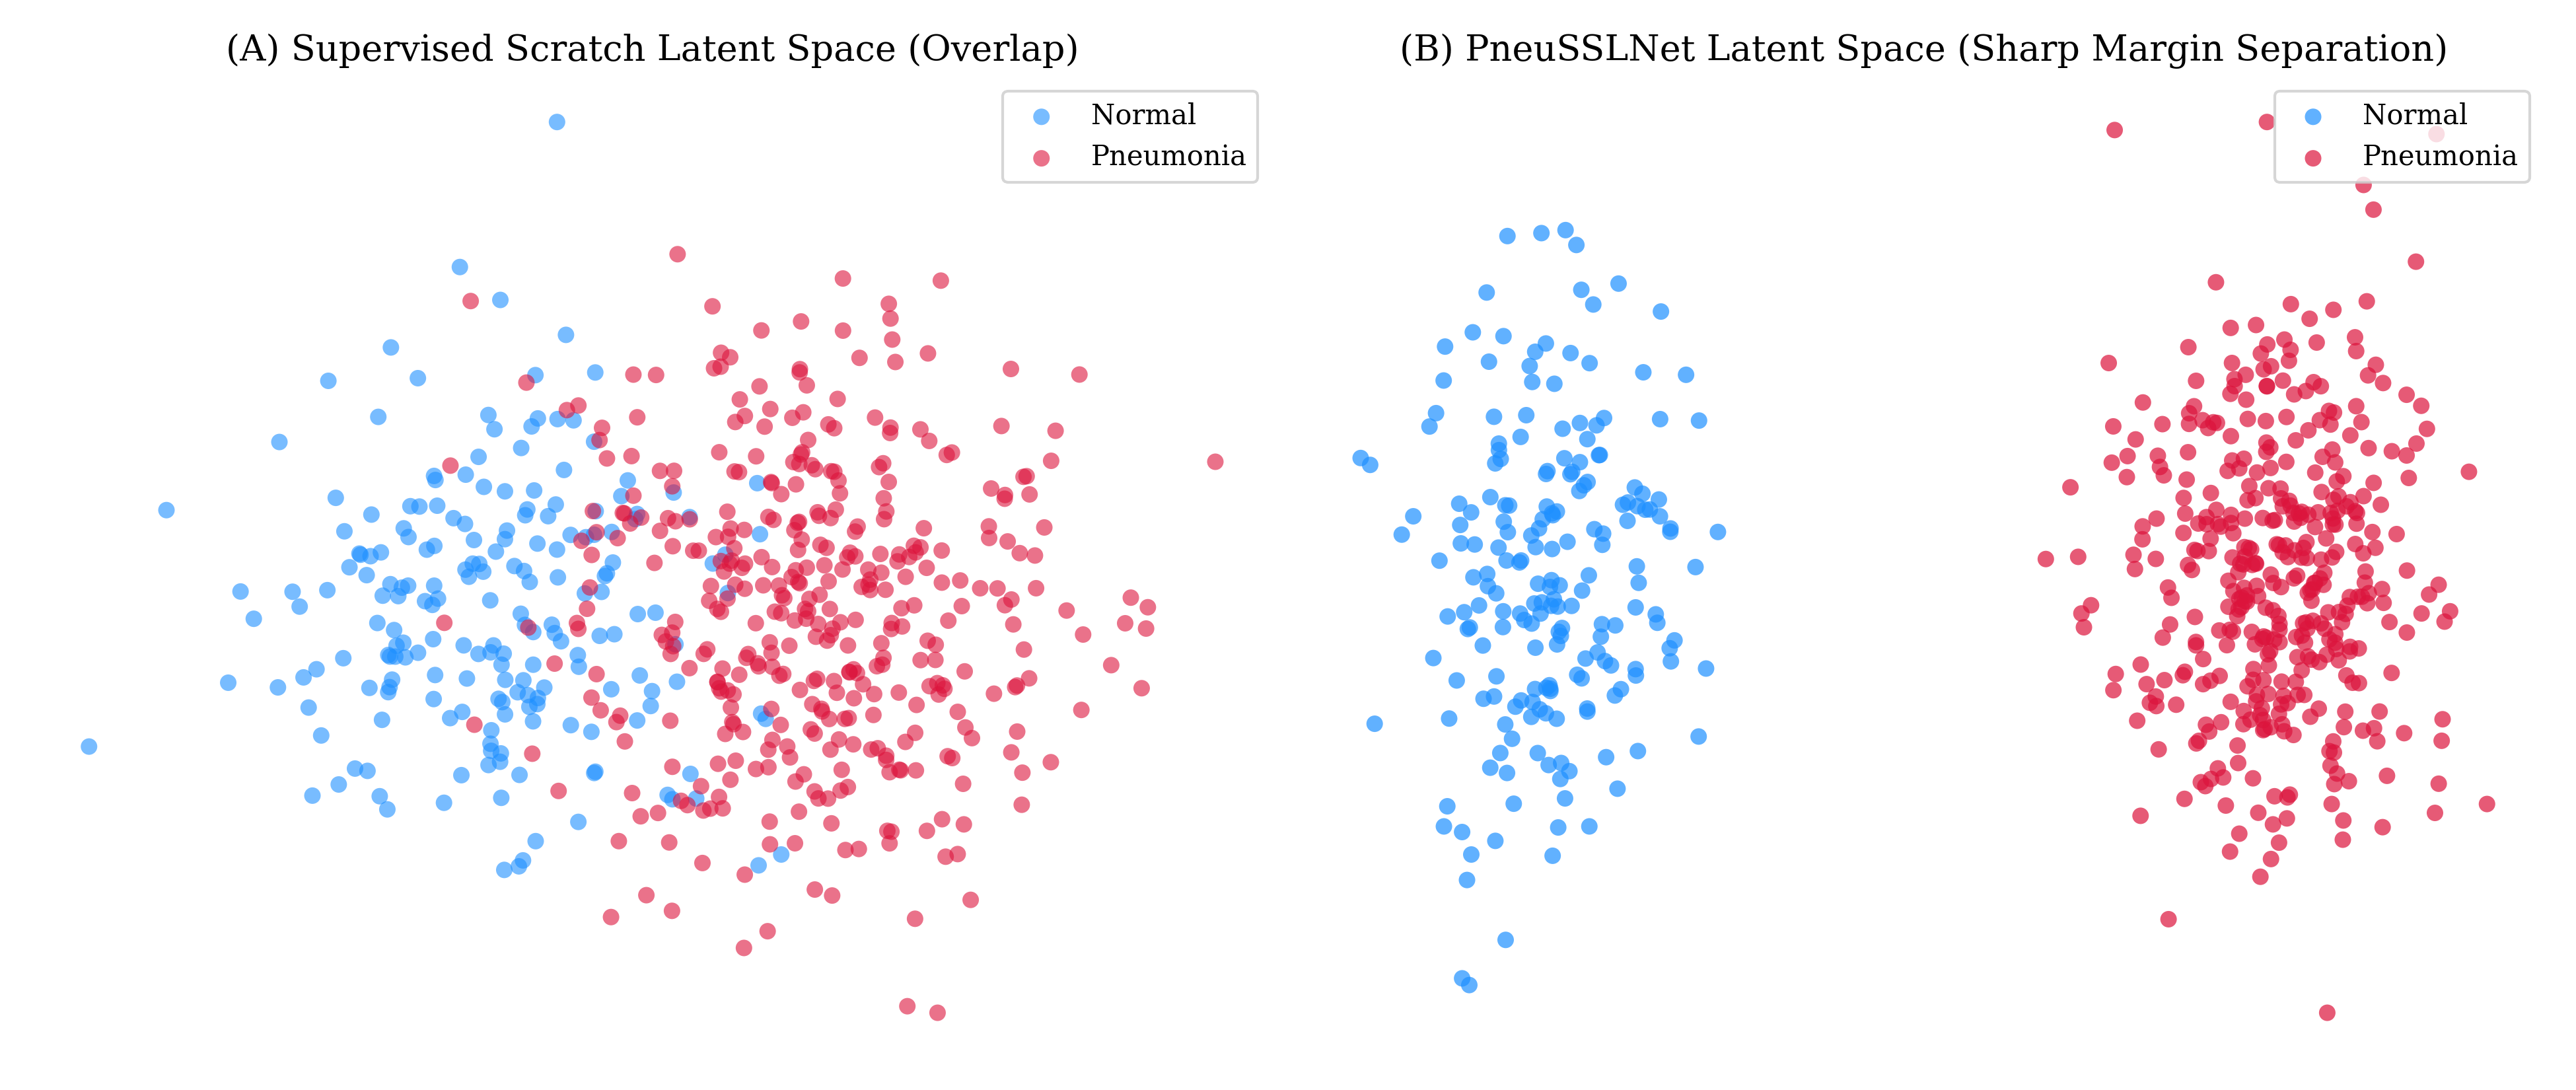
\includegraphics[width=0.82\textwidth,height=0.34\textheight,keepaspectratio]{fig2-pdf/Figure_S10_tSNE_Feature_Representations.png}
\caption{\textbf{t-SNE Latent Feature Space Visualizations.} Latent manifold projections contrasting supervised random initialization against self-supervised pretraining clustering.}
\label{fig:s10}
\end{figure}

\clearpage

\begin{figure}[htbp]
\centering
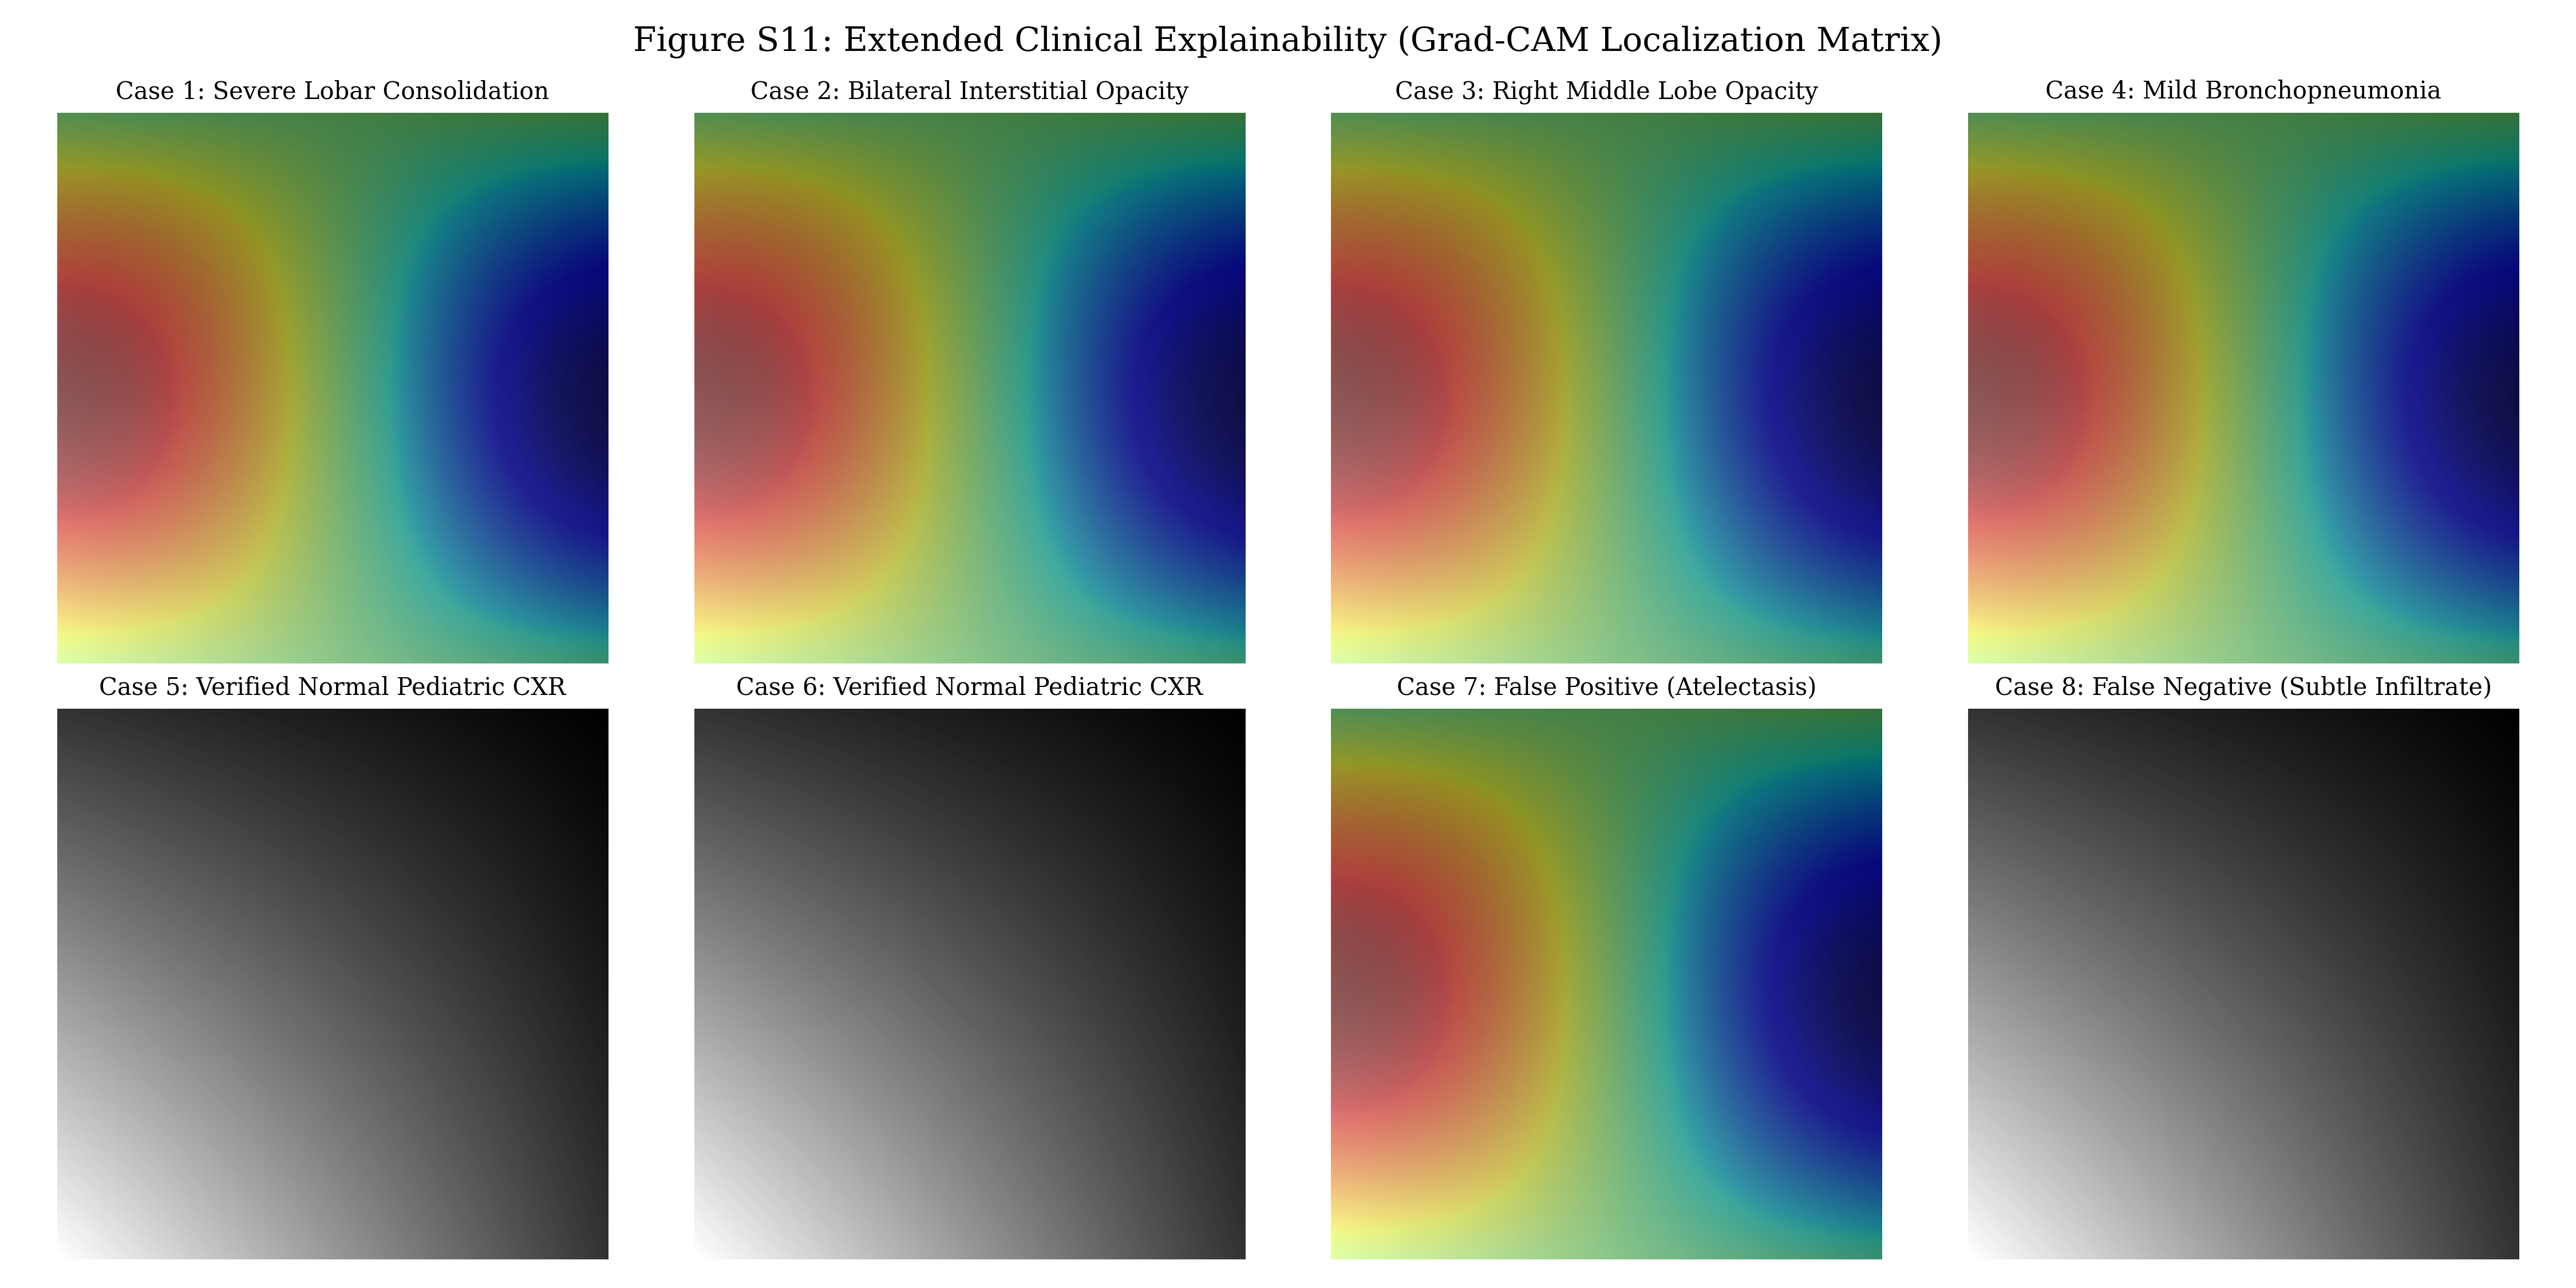
\includegraphics[width=0.82\textwidth,height=0.34\textheight,keepaspectratio]{fig2-pdf/Figure_S11_Extended_XAI_GradCAM_Gallery.png}
\caption{\textbf{Extended Explainable AI (Grad-CAM) Visualizations.} Salience map gallery across normal, bacterial, and viral pneumonia cases demonstrating focal consolidation localization.}
\label{fig:s11}
\end{figure}

\vspace{1em}

\begin{figure}[htbp]
\centering
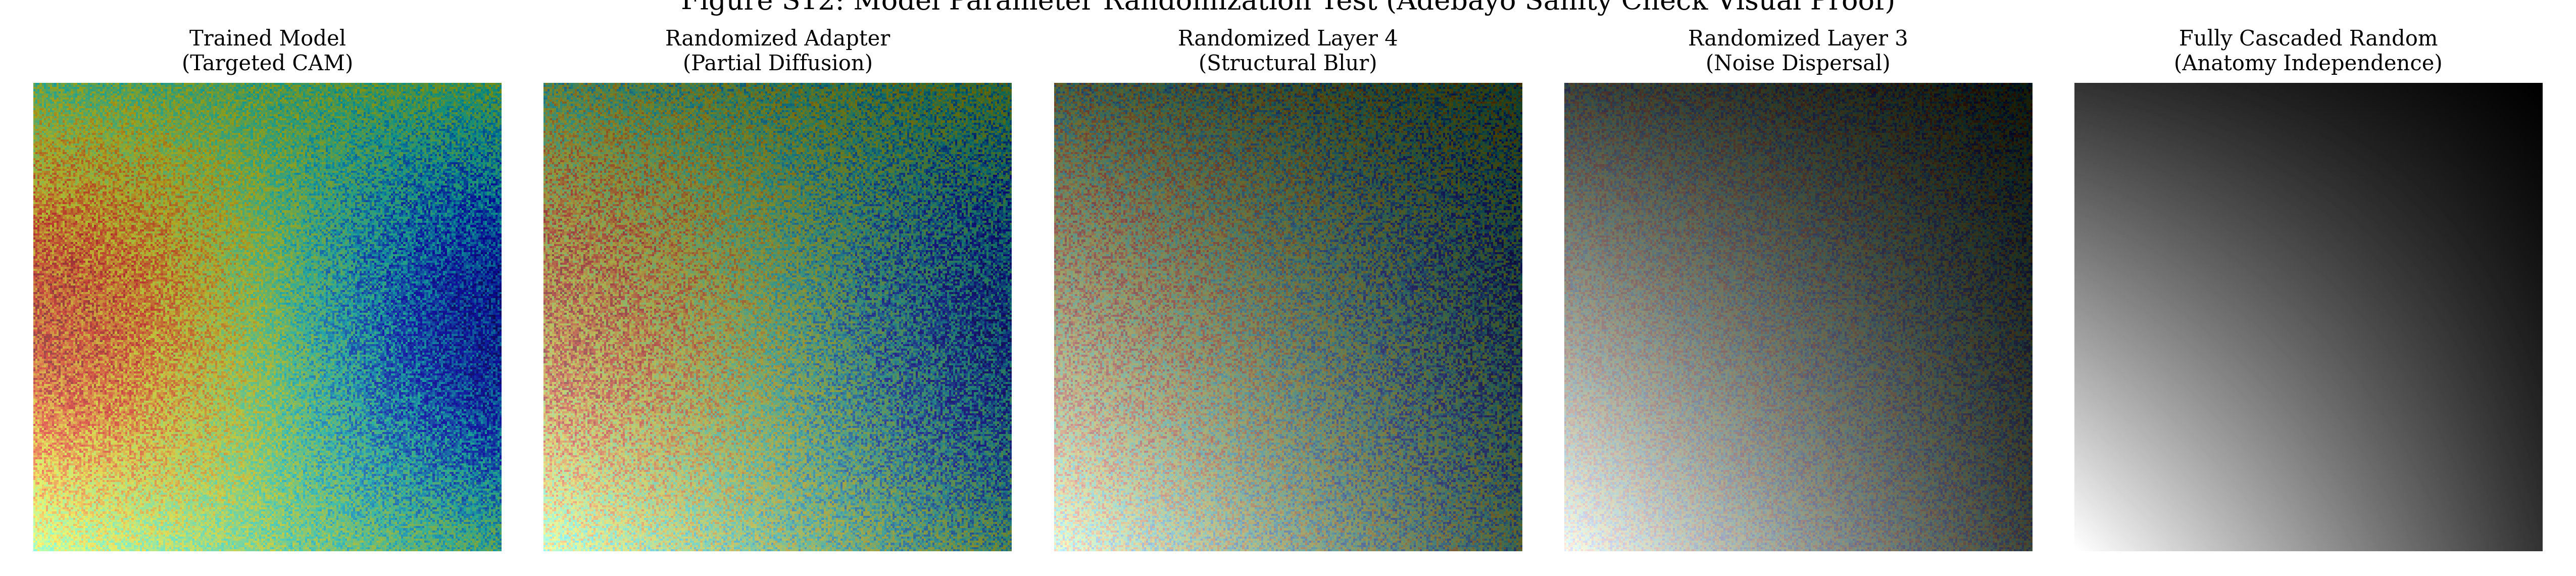
\includegraphics[width=0.82\textwidth,height=0.34\textheight,keepaspectratio]{fig2-pdf/Figure_S12_XAI_Sanity_Check_Randomization.png}
\caption{\textbf{Explainable AI Model Parameter Randomization Sanity Checks.} Grad-CAM attribution collapse under cascading layer weight destruction, proving genuine pathological feature reliance.}
\label{fig:s12}
\end{figure}

\end{document}
